\chapter{モジュール情報及び品質試験結果管理システム}\label{chap:dbsystem}
前章で述べたように、モジュール生産及び品質試験を世界中で行う。
これらの情報はデータベースシステムを用いて管理することが決定していて、現在この開発を行っている。
システムは、ITkの全情報を保存する中央データベースと、各組み立て機関に設置し、データ管理を行うローカルデータベースから成る。
本章ではこれらのデータベースについて説明する。また本研究における開発項目について詳細に説明する。

%%%%%%%%%%%%%%%%%%%%%%%%%%%%%%%%%%%%%%%%%%%%%%%%%
%%%%%%%%%%%%%%%%%%%%%%%%%%%%%%%%%%%%%%%%%%%%%%%%%
%%%%%%%%%%%%%%%%%%%%%%%%%%%%%%%%%%%%%%%%%%%%%%%%%
\section{中央データベース}
\subsection{中央データベースの概要}
\subsubsection{概要}
中央データベースは、ITkの製造に関する全ての情報の保存を目的として開発されたデータベースである。
ユニコーン大学が開発、運用を行っていて、チェコにデータベースサーバーが設けられている。
これらを生産するにあたって、シリコンセンサーやフレキシブル基板といった小さな部品から製造を行い、それらを用いたモジュールの組み立て、複数モジュールを搭載したステーブやリングの組み立てを経て検出器が完成する。
また各組み立て段階において、動作確認等を目的とした品質試験を行う。
これらの過程における全ての構成部品の情報、及び品質試験結果を中央データベースに保存する。

\subsubsection{意義}
中央データベースを扱う一番の目的は、ITkに用いるモジュールの選別とその配置の決定に用いることである。
品質試験結果を解析、品質のいいモジュールを選別、ITkに搭載する。
また、モジュール配置も品質を考慮して決定する。
例として以下の2つをあげる。
\begin{enumerate}
  \item $|\eta|$が小さい領域には、不良ピクセルが少なく品質の良いモジュールを搭載する.
  \item 不良ピクセルの領域が固まらないようにする.
\end{enumerate}
項目1に関して、ヒッグスなど物理解析で興味の対象となる粒子は相対的に大きい質量をもつため、ビーム軸方向に大きな運動量を持たず$|\eta|$の小さい領域域に生成される。
図\ref{VBF_image}のイベントディスプレイでも、ヒッグス粒子から生成される電子やミューオンが持つ$|\eta|$は小さいことが分かる。
そのため、$|\eta|$が小さい領域には品質の良いモジュールを配置する。
項目2に関して、不良ピクセルの領域がばらけるようにモジュールの配置を決定する。


次に中央データベースに保存された情報は、検出器運転時の参考値として扱われる。
モジュールを例にだすと、品質試験で読み出し試験を行った際の最適な設定値を中央データベースに保存するため、実際の運転時に参照することができる。
また運転前後での検出器性能比較を行うことができる。

%%%%%%%%%%%%%%%%%%%%%%%%%%%%%%%%%%%%%%%%%%%%%%%%%
%%%%%%%%%%%%%%%%%%%%%%%%%%%%%%%%%%%%%%%%%%%%%%%%%
%%%%%%%%%%%%%%%%%%%%%%%%%%%%%%%%%%%%%%%%%%%%%%%%%
\section{ローカルデータベース}
\subsection{ローカルデータベースの意義と概要}
中央データベースでは、前述したようにモジュール情報のみならずITkの製造に関わるすべての情報を管理する。
データベースの機能としては、製造を通して汎用的に使えるものになっている。
モジュールの組み立て及びその品質試験に関しては\ref{chap:qc_test}章で述べたように工程が複数に渡り、行う品質試験の数も多い。
1つの組み立て機関で多いところでは数千個のモジュールを作ることになるため、
データ管理が簡単にかつ円滑に進むようになっているのが好ましい。
このような理由から、組み立て機関での生産性、利便性に特化し、円滑な生産をサポートすることを目的としたデータベースシステムを開発しており、これを「\textbf{ローカルデータベース}」と呼ぶ。
システムの概要図を図\ref{localdb_overview}に示す。オープンソースのサービスであるMongoDB\cite{4-1}と、
PythonのウェブフレームワークであるFlask\cite{4-3}を使用して開発を行なっているローカルデータベース用ウェブアプリケーションを併用することで、データ管理や中央データベースとの同期を行うシステムとなっている。

ローカルデータベースシステムは以下のような利点を持ち得る。
これらの利点を持つシステムの開発、実装を行うことが開発課題となっている。

\begin{itemize}
  \item ローカルにデータベースサーバーを立てるため通信速度が早く、円滑にデータ管理を行うことができる。
  \item モジュールの組み立て工程を管理し、生産者の適切な処理を助ける。
  \item モジュールに特化したデータ管理、結果解析を行うことで異常をいち早く検知できる。
  \item 試験者情報や試験時間など、品質試験結果以外の必要な情報を正確に管理できる。
\end{itemize}

一方で欠点として、ローカルデータベースと中央データベース間で同期とその管理を行う必要があることがあげられる。
この問題は以下により解決する。それぞれの詳細については後述する。
\begin{itemize}
  \item 同期ツールの開発.
  \item データベース操作の流れの確立.
  \item 操作方法の普及に向けたチュートリアル、ドキュメント作成.
\end{itemize}

\begin{figure}[bpt]\centering
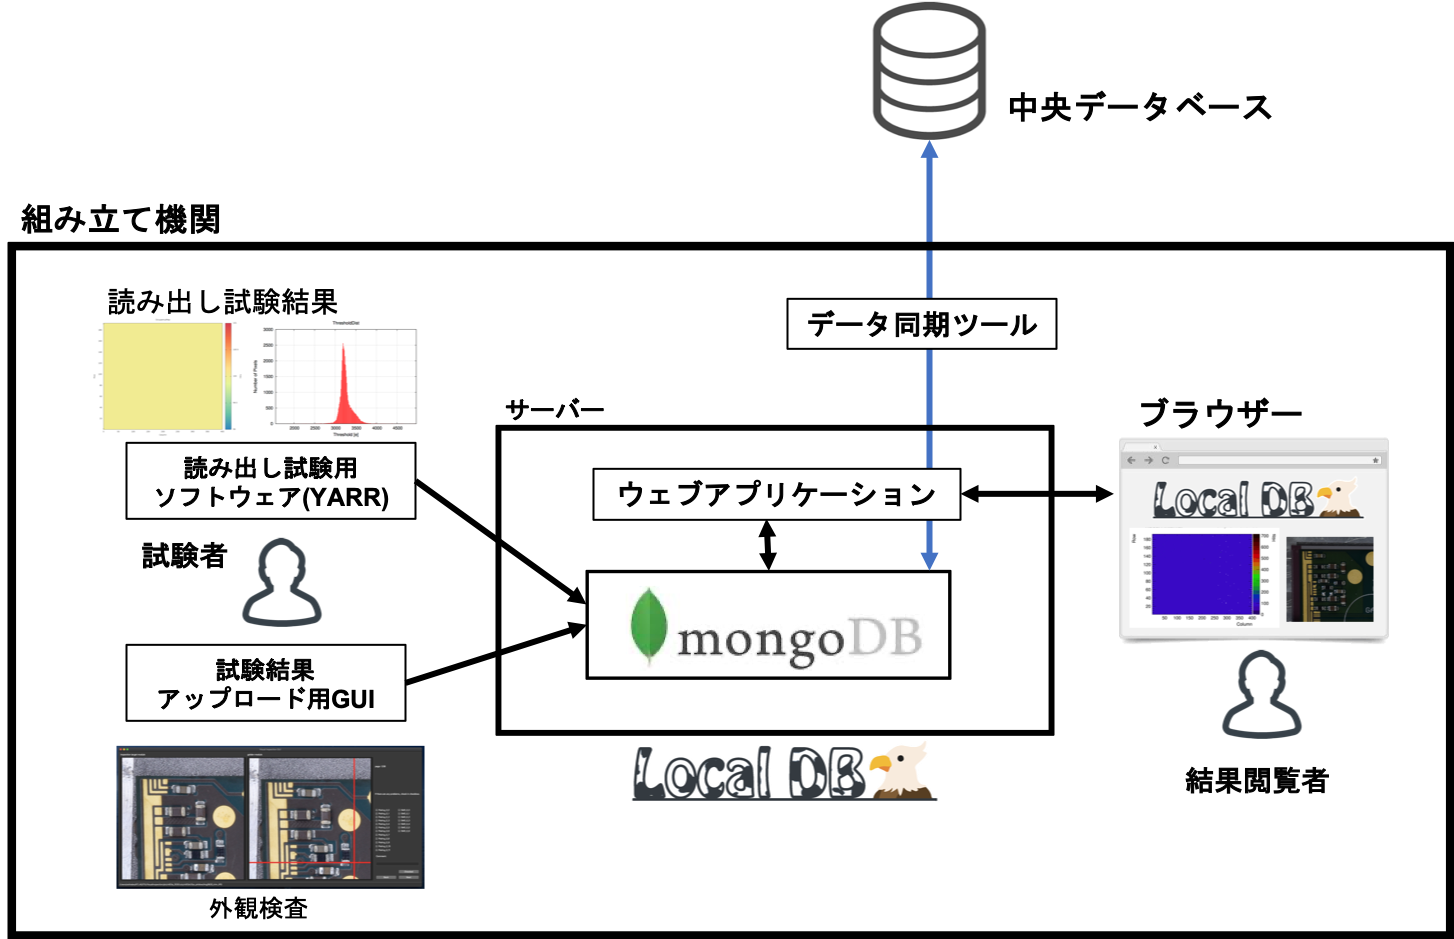
\includegraphics[width=12cm]{./localdb_overview.png}
\caption[ローカルデータベースシステムの概要]{ローカルデータベースシステムの概要。各組み立て機関でMongoDBとローカルデータベース用ウェブアプリケーションの立ち上げを行い、独自にデータ管理をするシステムとなっている。ウェブアプリケーションにはPythonパッケージであるFlaskを使用している。品質試験者は図のようにいくつかのソフトウェアを用いて試験結果をMongoDBに保存する。保存された結果はウェブアプリケーションによって閲覧することができる。また結果は中央データベースに集める必要があるため、同期ツールを用いて試験結果の共有を行う。}
\label{localdb_overview}
\end{figure}

\subsection{先行研究と開発課題}
先行研究で開発された領域と、本研究で取り組んだ開発課題を以下に示す。

\subsubsection{先行研究}
先行研究\cite{4-6}においてデータベースシステムの設計と開発がなされ、図\ref{localdb_overview}におけるいくつかの項目が開発された。
以下に実装項目を記す。
\begin{enumerate}
  \item 読み出し試験結果保存のためのMongoDB内部構造の設計.
  \item 1の構造を用いてYARRからMongoDBへの読み出し試験結果アップロード機能.
  \item 試験結果のソート及び閲覧が可能な、Flaskを用いたウェブアプリケーション. 
\end{enumerate}

モジュールの生産、品質試験に向けたデータ管理、そしてローカルデータベースの利点を活かすには以下のような開発課題が残されていた。
\begin{itemize}
  \item 中央データベースの内部構造の実装.
  \item 中央データベースとローカルデータベース間の同期ツールの開発.
  \item ローカルデータベースにおける品質試験に特化したデータ管理と機能提供.
  \item 量産時におけるデータベース操作の流れの確立.
\end{itemize}

これらの開発課題に対して、本研究で取り組んだ項目を以下に挙げる。
なお先行研究で開発したデータ構造やアプリケーションといった項目は既に複数の機関で試験運用されていたため、本研究ではその構造やソフトウェアを大きく変更せずに、拡張する形で開発を行なった。

\subsubsection{中央データベースの内部構造の実装}
モジュール及び品質試験の結果を中央データベースに登録するために、モジュールの種類や品質試験項目など中央データベースにおける内部構造の実装する必要がある。本研究ではこういった量産時において必要となるデータ構造の実装を行なった。

\subsubsection{中央データベースとローカルデータベース間の同期ツールの開発}
ローカルデータベースを各組み立て機関に設置し、データ管理を行う。
中央データベースに必要な情報が全て保存されるためにはデータベース間の同期が必要である。
これを達成するために中央データベースとローカルデータベースの同期を行うツール開発を行なった。

\subsubsection{ローカルデータベースにおける品質試験に特化したデータ管理と機能提供}
ローカルデータベースの利点を活かすため、「品質試験に特化したデータ管理と機能提供」を目的として以下の機能を実装した。
\begin{itemize}
  \item 品質試験者及びシステムユーザ管理機能及びコメント付加等の各種ユーザ機能.
  \item 品質試験結果の登録と組み立て工程の自動更新.
  \item 読み出し試験におけるピクセル解析ツールの開発.
  \item 読み出し試験結果の検索機能.
\end{itemize}

\subsubsection{量産時におけるデータベース操作の流れの確立}
実際のモジュール組み立て時には品質試験結果の登録、同期といったデータベース操作を正しい流れで行う必要がある。
この操作の流れが確立されていなかっため、本研究では上述した機能開発と併せて品質試験におけるデータベース操作の流れを確立した。

%%%%%%%%%%%%%%%%%%%%%%%%%%%%%%%%%%%%%%%%%%%%%%%%%
%%%%%%%%%%%%%%%%%%%%%%%%%%%%%%%%%%%%%%%%%%%%%%%%%
%%%%%%%%%%%%%%%%%%%%%%%%%%%%%%%%%%%%%%%%%%%%%%%%%
\clearpage
\subsection{MongoDBと内部構造\cite{4-2}}
MongoDBとはNoSQLに分類されるデータベースである。
MongoDBの構造について簡単に表したものを図\ref{mongodb_schema}に示す。
一般的なSQLDBのようにテーブル形式ではなく、JSON形式で情報を格納する。
情報を保持している一枚のJSONインスタンスを「\textbf{ドキュメント}」と呼び、「\textbf{コレクション}」と呼ばれる枠に複数のドキュメントが格納されている。
各ドキュメントは「\textbf{ID}」と呼ばれるハッシュ値を持っていて、異なるコレクションにおけるドキュメント間の紐付けはこのIDを用いて行う。

\begin{figure}[bpt]\centering
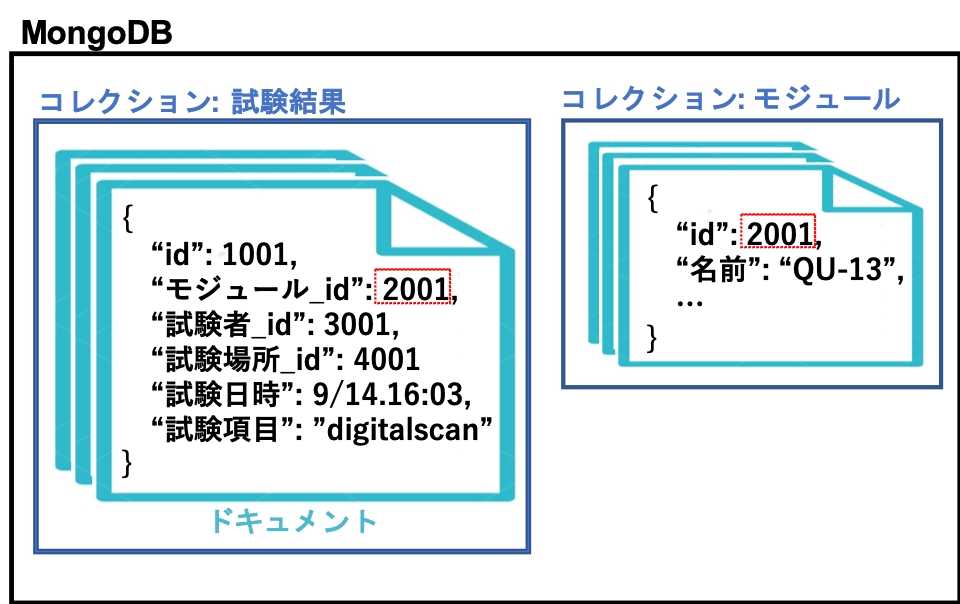
\includegraphics[width=12cm]{./mongodb_schema.png}
\caption[MongoDBの構造の例\cite{4-2}]{MongoDBの構造の例\cite{4-2}。図のようにMongoDBではJSON形式でデータを格納する。1枚のJSONインスタンスをドキュメントと呼び、複数のドキュメントが格納されている枠組みをコレクションと呼ぶ。ドキュメントの構造及びコレクション間の関係等を決めることでデータベースの構造を定義する。ドキュメント間の紐付けは、各ドキュメント内部にIDを持つことで可能となる。図の例では試験結果のドキュメントが$\{$``モジュール$\_$id":2001$\}$の情報を持っており、これがモジュールに保存されているドキュメントのIDに対応する。}
\label{mongodb_schema}
\end{figure}


ローカルデータベースシステムにおいて、MongoDBを使用する主な利点を以下に示す。

\begin{itemize}
  \item 各コレクションに格納するドキュメントの構造が動的であるため、開発を柔軟に行うことができる。
  \item JSON形式でデータを保持するため情報取得の際の整形処理が容易であり、ウェブアプリケーションとの親和性が高い。
  \item データのキャッシュをメモリ上に置き処理を実行するため、高速な読み書きが可能\cite{4-8}。
\end{itemize}

モジュール及び品質試験に用いる主なコレクションを表\ref{localdb_structure}に示す。
また先行研究で設計された読み出し試験結果に関する内部構造を図\ref{localdb_structure_detail}に示す。

%%%%%%%%%%%%%%%%%%%%%%%%%%%%%%%%%%%%%%%%%%%%%%%%%
%%%%%%%%%%%%%%%%%%%%%%%%%%%%%%%%%%%%%%%%%%%%%%%%%
%%%%%%%%%%%%%%%%%%%%%%%%%%%%%%%%%%%%%%%%%%%%%%%%%
\begin{table}[btp]
\begin{center}
\caption[品質試験に用いる主なコレクション]{品質試験に用いる主なコレクション。ローカルデータベースシステムにおいて、MongoDB内に2つのデータベースを設置し、使用する。}
\label{localdb_structure}
  \small
  \begin{tabular}{|lll|} \hline
    データベース名 & コレクション名 & 情報 \\ \hline
    localdb      & component & モジュール情報、FEチップ情報 \\ 
                 & childParentRelation & FEチップとモジュールの関係性 \\ 
                 & QC.module.status & 各モジュールに対する組み立て工程及び選択された試験結果 \\ 
                 & QC.result & 品質試験結果 \\ 
                 & testRun & 読み出し試験結果 \\ 
                 & user & 読み出し試験実施者 \\
                 & institute & 読み出し試験実施場所 \\
                 & componentTestRun & componentとtestRunの関係性 \\
                 & comments & コメント情報 \\ \hline
    localdbtools & QC.status & 組み立て工程及び試験項目\\
                 & viewer.user & 登録ユーザの情報 \\
                 & viewer.query & 読み出し結果キーワード、検索機能実行時に使用 \\ 
                 & viewer.tag.docs & モジュールや試験結果に付けるタグの情報 \\ \hline
  \end{tabular}
\end{center}
\end{table}

\begin{figure}[bpt]\centering
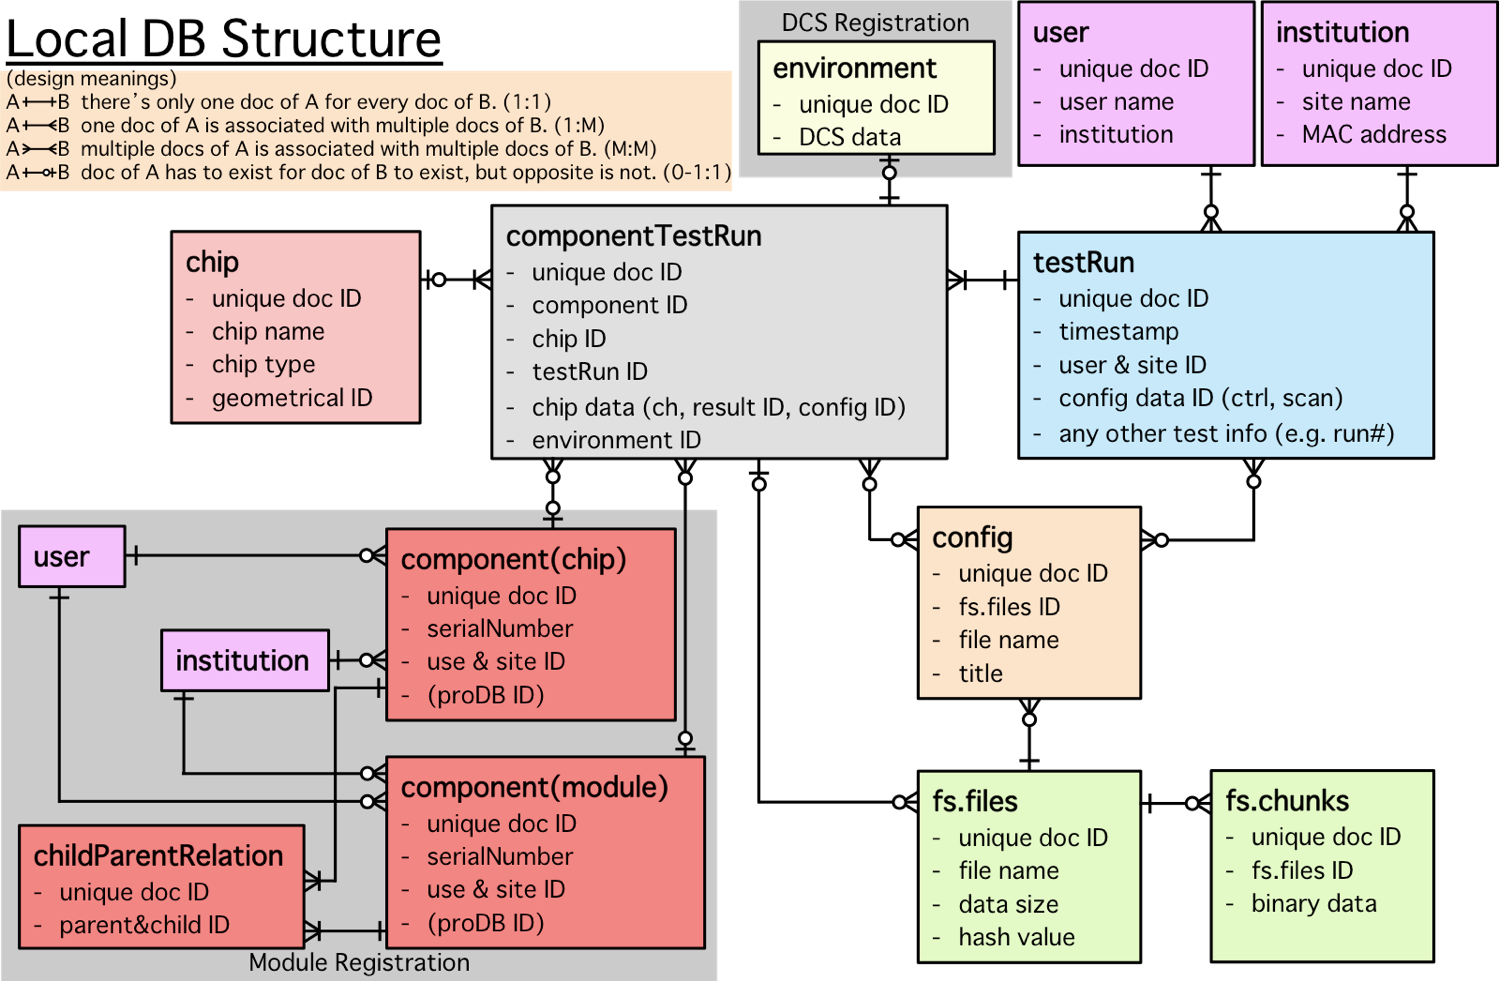
\includegraphics[width=12cm]{./localdb_structure_detail.png}
\caption[先行研究により設計された読み出し試験結果のMongoDB内部構造]{先行研究により設計された読み出し試験結果のMongoDB内部構造\cite{4-6}。それぞれの四角はコレクション、直線はIDによるドキュメント間のリンクを示している。直線が十字になっている場合は対応するドキュメントが1つであることを示し、分岐しているものは複数であることを示す。また直線状の白丸は対応するドキュメントが存在しない場合があることを示している。}
\label{localdb_structure_detail}
\end{figure}

\clearpage
%%%%%%%%%%%%%%%%%%%%%%%%%%%%%%%%%%%%%%%%%%%%%%%%%
%%%%%%%%%%%%%%%%%%%%%%%%%%%%%%%%%%%%%%%%%%%%%%%%%
%%%%%%%%%%%%%%%%%%%%%%%%%%%%%%%%%%%%%%%%%%%%%%%%%
\subsection{ウェブアプリケーション} \label{sec:web_app}

各組み立て機関において、試験者が品質試験結果を閲覧、管理するツールとして、ウェブアプリケーションを提供している。
アプリケーション開発には、PythonのウェブフレームワークであるFlaskを使用している。
またアプリーケーションにおいてMongoDBとの通信に用いるAPIとして、PythonライブラリであるPyMongo\cite{4-4}を用いている。
アプリケーション処理に特化したイメージを図\ref{webapp_process}に示す。
このようにアプリケーションはデータベースとブラウザー、データベース間のインターフェースとなっている。

試験結果を迅速に分かりやすく見るシステムを作り、円滑な生産補助や異常結果の早期発見を目的としている。
またデータベースの情報管理のみならず、同期ツールや、後述する試験結果解析ツールなどの外部スクリプトの実行、結果取得等、生産時における多くのデータベース操作はこのアプリケーションを用いて行う。

ウェブアプリケーションでは、現在以下の機能を使用することができる。ある品質試験の結果ページを図\ref{viewer_result}に示す。
\begin{itemize}
  \item 登録モジュール情報及び品質試験結果の閲覧、解析.
  \item ローカルデータベースにおけるユーザ管理機能.
  \item データベース同期実行機能.
\end{itemize}

\begin{figure}[bpt]\centering
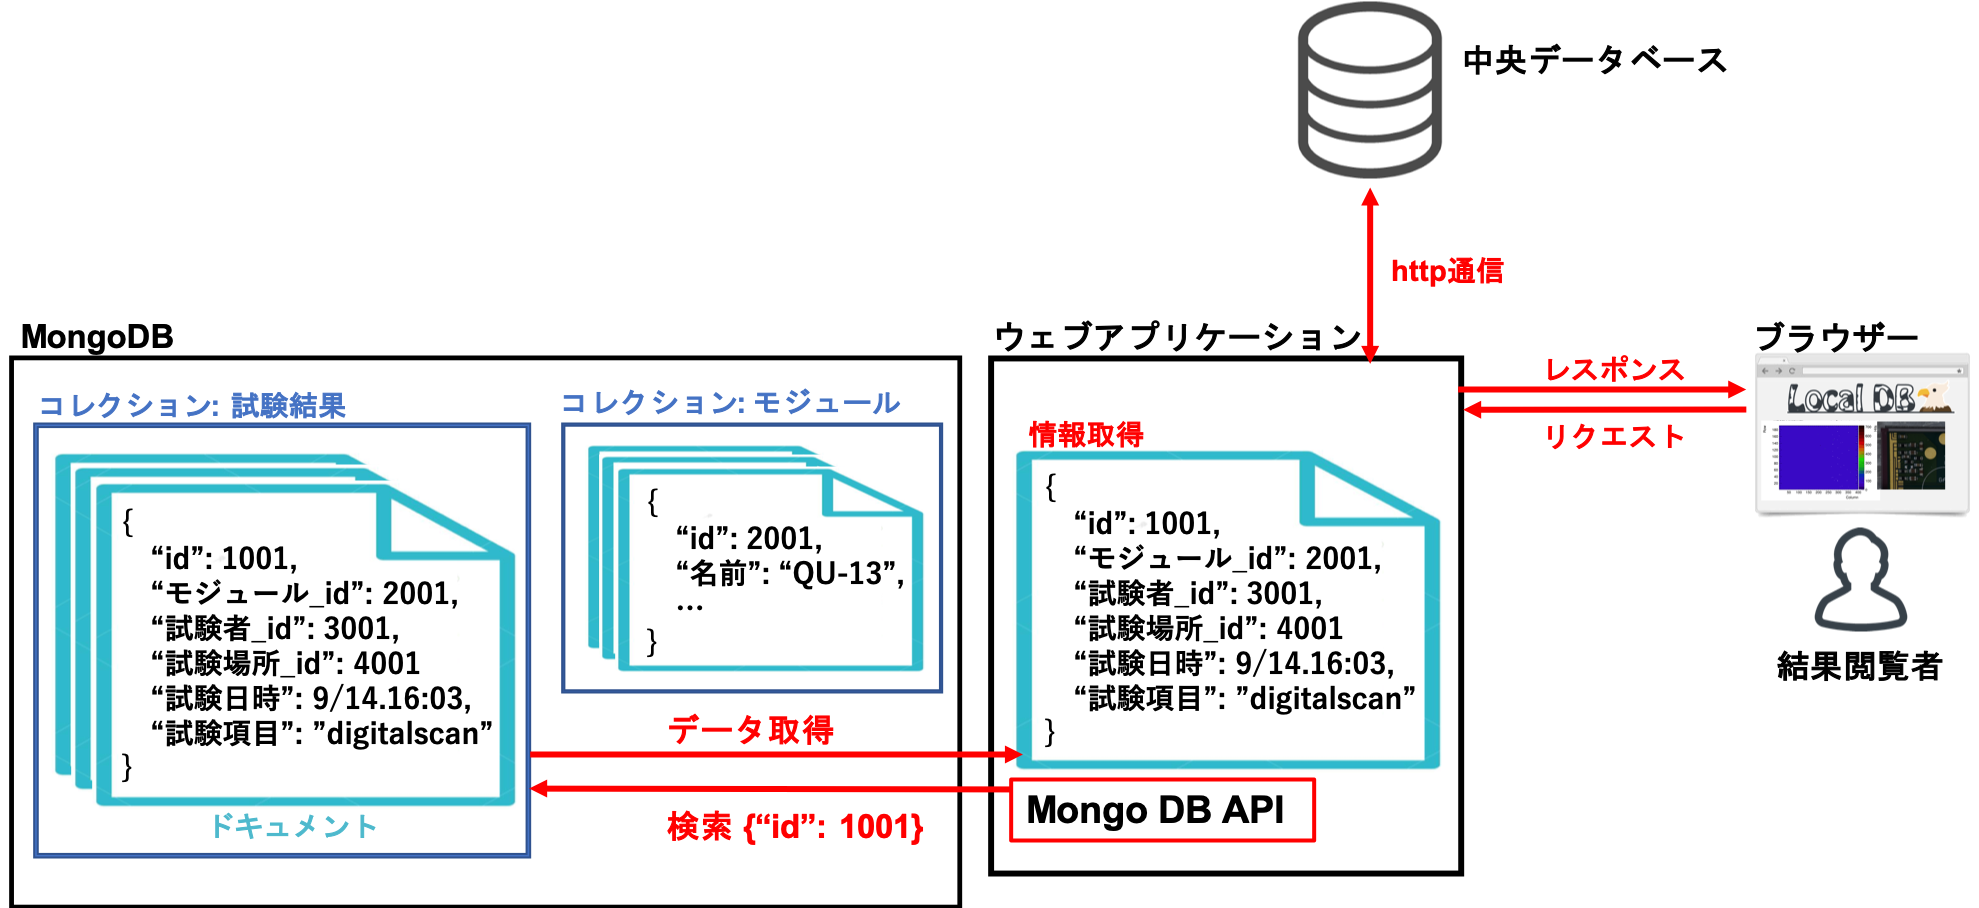
\includegraphics[width=16cm]{./webapp_process.png}
\caption[ウェブアプリケーション処理のイメージ]{ウェブアプリケーション処理のイメージ。ウェブアプリケーションではMongoDBと通信を行うAPI(PyMongo)を用いて、データベースのコレクションに検索をかけることで情報を取得する。取得した情報は整形されたのちブラウザに送信、中央データベースとの同期等の処理に用いられる。}
\label{webapp_process}
\end{figure}

\begin{figure}[bpt]\centering
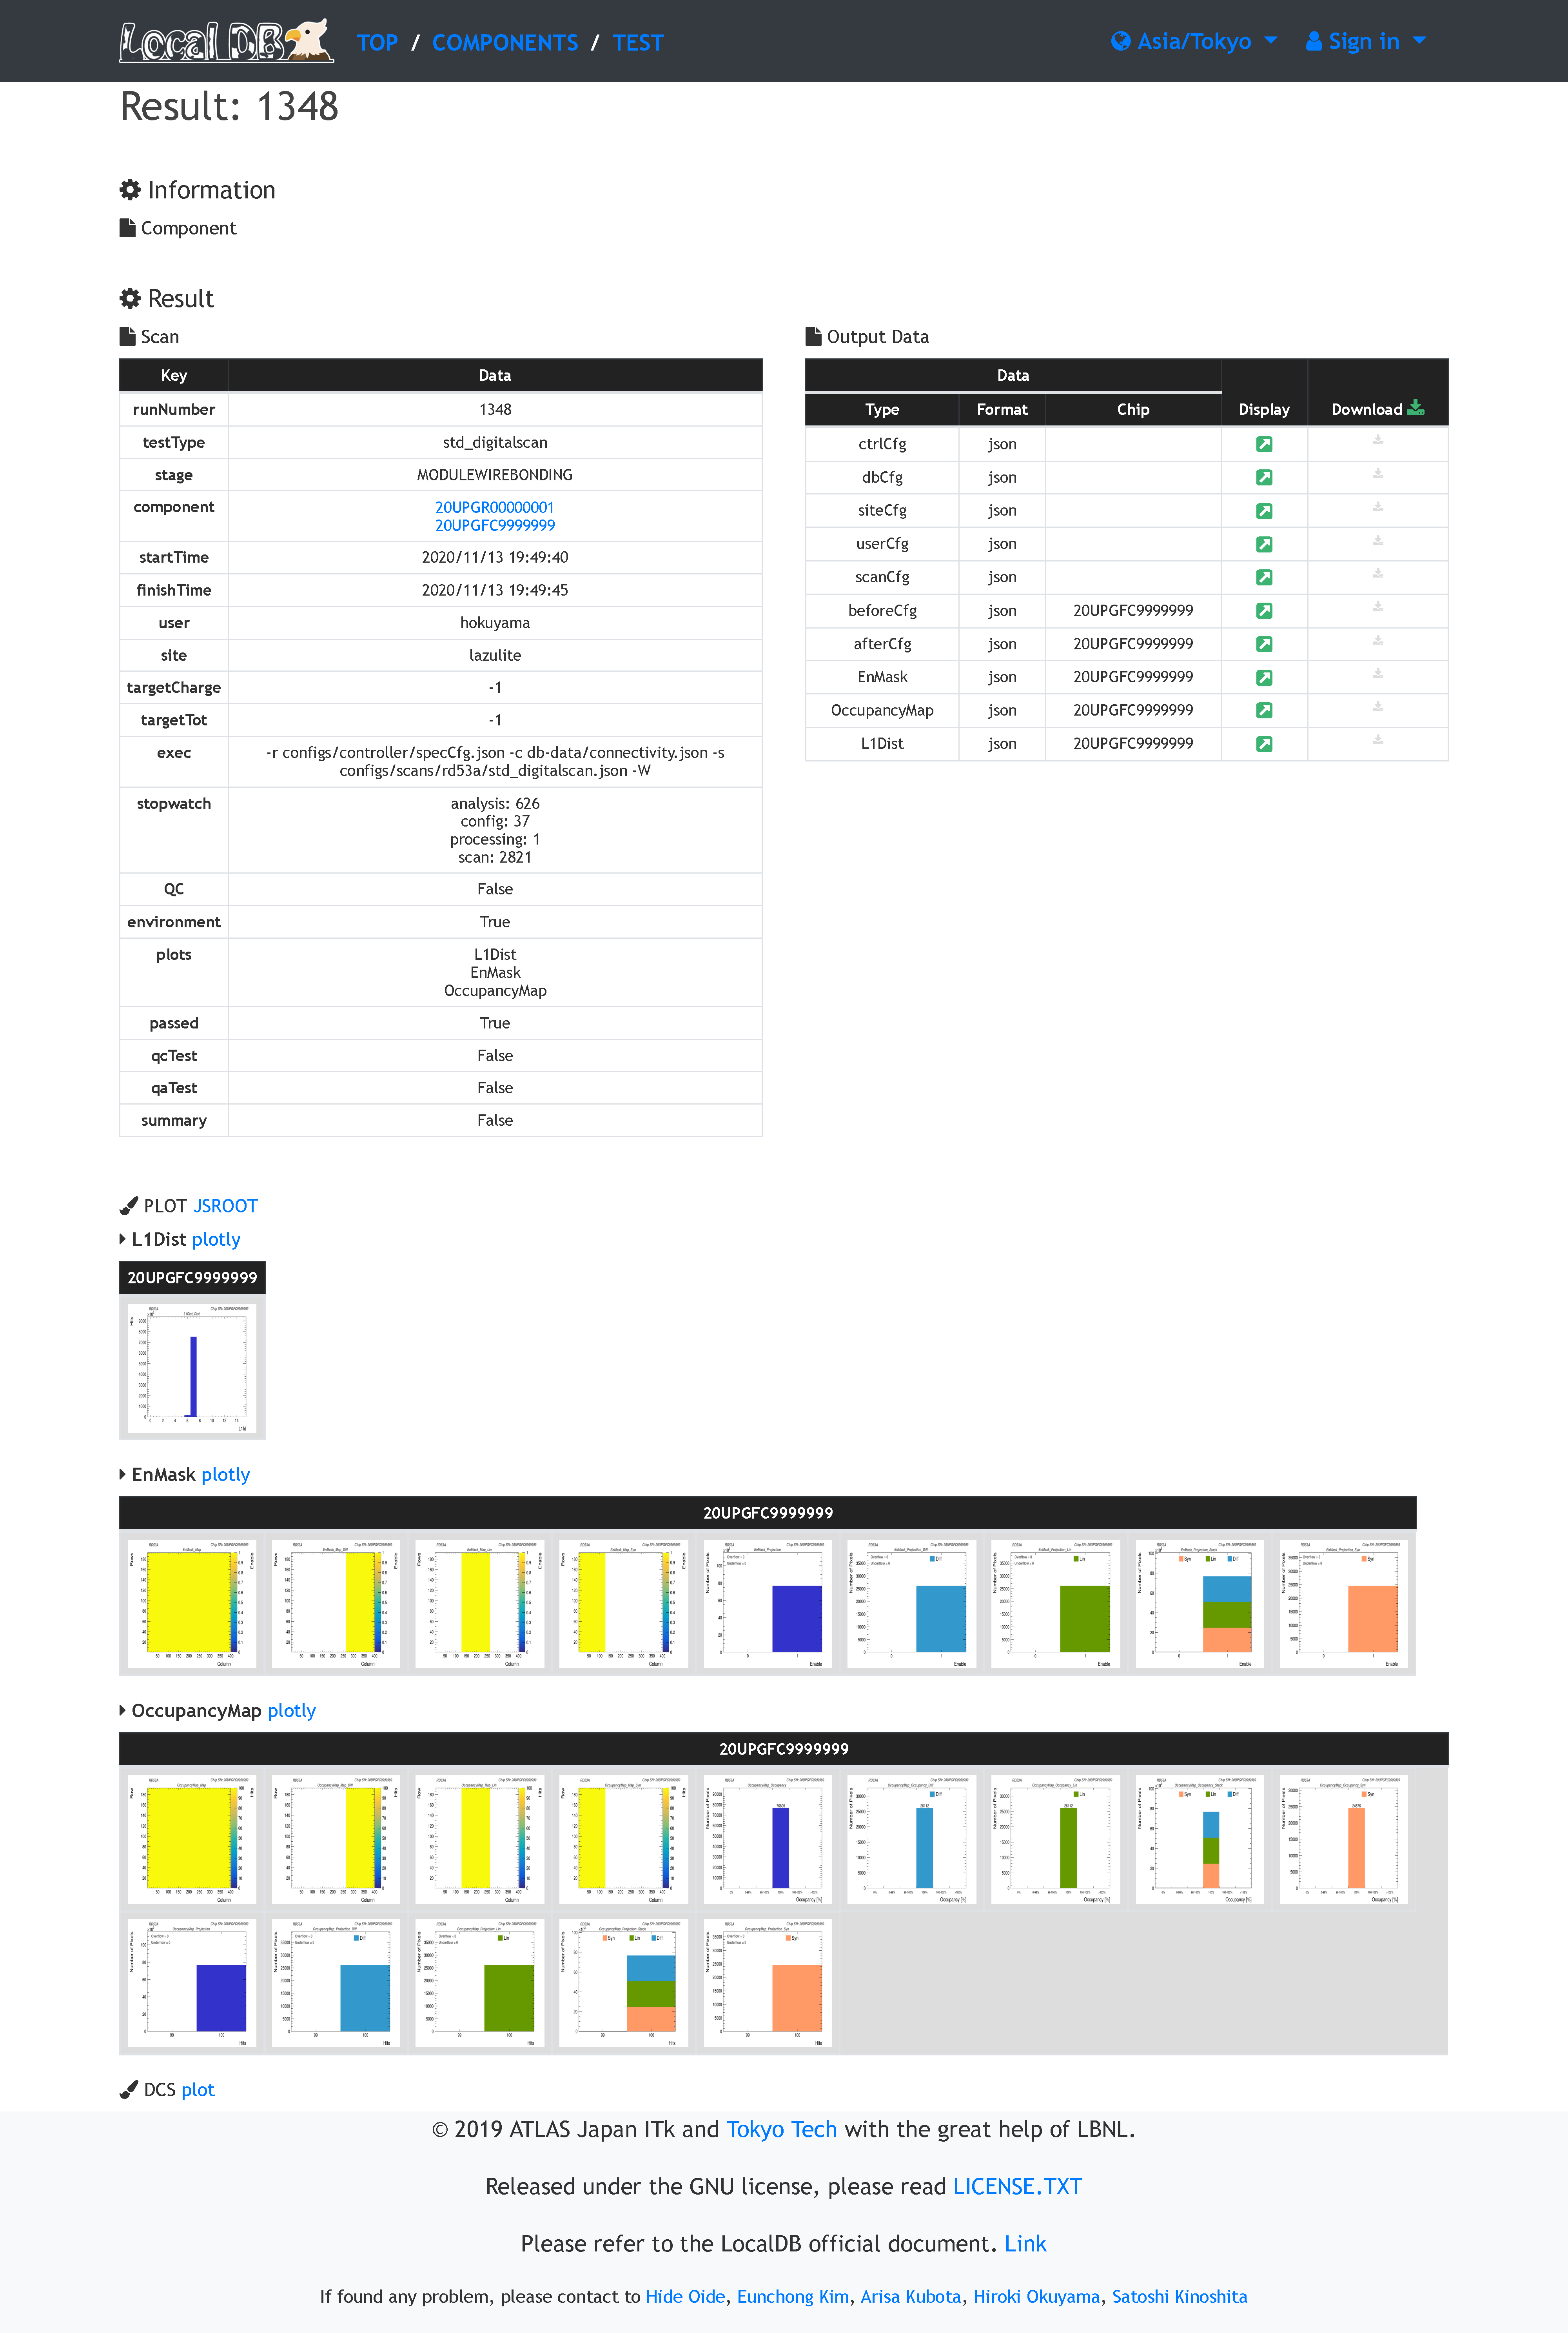
\includegraphics[width=15cm]{./demo_view_scan_result.pdf}
\caption[品質試験結果ページの例]{品質試験結果ページの例。図は品質試験項目であるデジタル回路読み出しの結果を表している。図の上部に試験情報や設定値、下部に結果のグラフが表示されているのを確認できる。}
\label{viewer_result}
\end{figure}


\clearpage
%%%%%%%%%%%%%%%%%%%%%%%%%%%%%%%%%%%%%%%%%%%%%%%%%%%
%%%%%%%%%%%%%%%%%%%%%%%%%%%%%%%%%%%%%%%%%%%%%%%%%%%
%%%%%%%%%%%%%%%%%%%%%%%%%%%%%%%%%%%%%%%%%%%%%%%%%%%
\section{本研究における開発項目の詳細}
以下は本研究で開発した項目である。

%%%%%%%%%%%%%%%%%%%%%%%%%%%%%%%%%%%%%%%%%%%%%%%%%%%
%%%%%%%%%%%%%%%%%%%%%%%%%%%%%%%%%%%%%%%%%%%%%%%%%%%
%%%%%%%%%%%%%%%%%%%%%%%%%%%%%%%%%%%%%%%%%%%%%%%%%%%
\subsection{中央データベースの内部データ構造の実装}

モジュール及びその品質試験に関する情報を中央データベースに保存するために、情報構造の定義、実装を行う必要がある。
以下の項目について、中央データベースが提供しているAPIを用いて構造の定義を行った。
\begin{enumerate}
  \item モジュールの種類とその構成部品(図\ref{pd_module_structure}).
  \item モジュール組み立て工程と付随する品質試験(表\ref{pd_stage_structure}).
\end{enumerate}

また項目1に関して、Quadモジュールに関する例を図\ref{example_module_structure}に示す。

%\begin{table}[b]
%\begin{center}
%\caption[中央データベースにおけるモジュールの種類と構造一覧]{中央データベースにおけるモジュールの種類と構造一覧。中央データベースにモジュールを登録するときの情報として、モジュールの種類、構成部品を表のように実装した。Triplet、Quadというように、モジュールの種類ごとに登録できるシステムとなっており、PCB(フレキシブル基板)などの対応する構成部品の紐付けも同時に行うことができる。}
%\label{pd_module_structure}
%  \scriptsize
%  \begin{tabular}{|ll|} \hline
%    種類 & 構成する部品(数) \\ \hline
%    Triplet L0 stave module   &  Single bare module(3) \\
%                              &  Triplet stave PCB(1) \\\hline
%    Triplet L0 Ring0 module   &  Single bare module(3) \\
%                              &  Triplet R0 PCB(1) \\\hline
%    Triplet L0 Ring0.5 module &  Single bare module(3) \\
%                              &  Triplet R0.5 PCB(1) \\\hline
%    L1 quad module            &  Quad bare module(1) \\
%                              &  Quad PCB(1) \\\hline
%    Outer system quad moudle  &  Quad bare module(1) \\
%                              &  Quad PCB(1) \\\hline
%    Outer system quad moudle  &  Dual bare module(1) \\
%                              &  Dual PCB(1) \\\hline
%    Digital triplet L0 stave module   &  Digital single bare module(3) \\
%                                      &  Triplet stave PCB(1) \\\hline
%    Digital triplet L0 Ring0 module   &  Digital single bare module(3) \\
%                                      &  Triplet R0 PCB(1) \\\hline
%    Digital triplet L0 Ring0.5 module &  Digital single bare module(3) \\
%                                      &  Triplet R0.5 PCB(1) \\\hline
%    Digital quad module       &  Digital quad bare module(1) \\
%                              &  Quad PCB(1) \\\hline
%    Digital L1 quad moudle    &  Digital quad bare module(1) \\
%                              &  Quad PCB(1) \\\hline
%    Dummy triplet L0 stave module   &  Dummy single bare module(3) \\
%                                    &  Triplet stave PCB(1) \\\hline
%    Dummy triplet L0 Ring0 module   &  Dummy single bare module(3) \\
%                                    &  Triplet R0 PCB(1) \\\hline
%    Dummy triplet L0 Ring0.5 module &  Dummy single bare module(3) \\
%                                    &  Triplet R0.5 PCB(1) \\\hline
%    Dummy quad module       &  Dummy quad bare module(1) \\
%                            &  Quad PCB(1) \\\hline
%    Dummy L1 quad moudle    &  Dummyl quad bare module(1) \\
%                            &  Quad PCB(1) \\ \hline
%  \end{tabular}
%\end{center}
%\end{table}

\begin{figure}[b]\centering
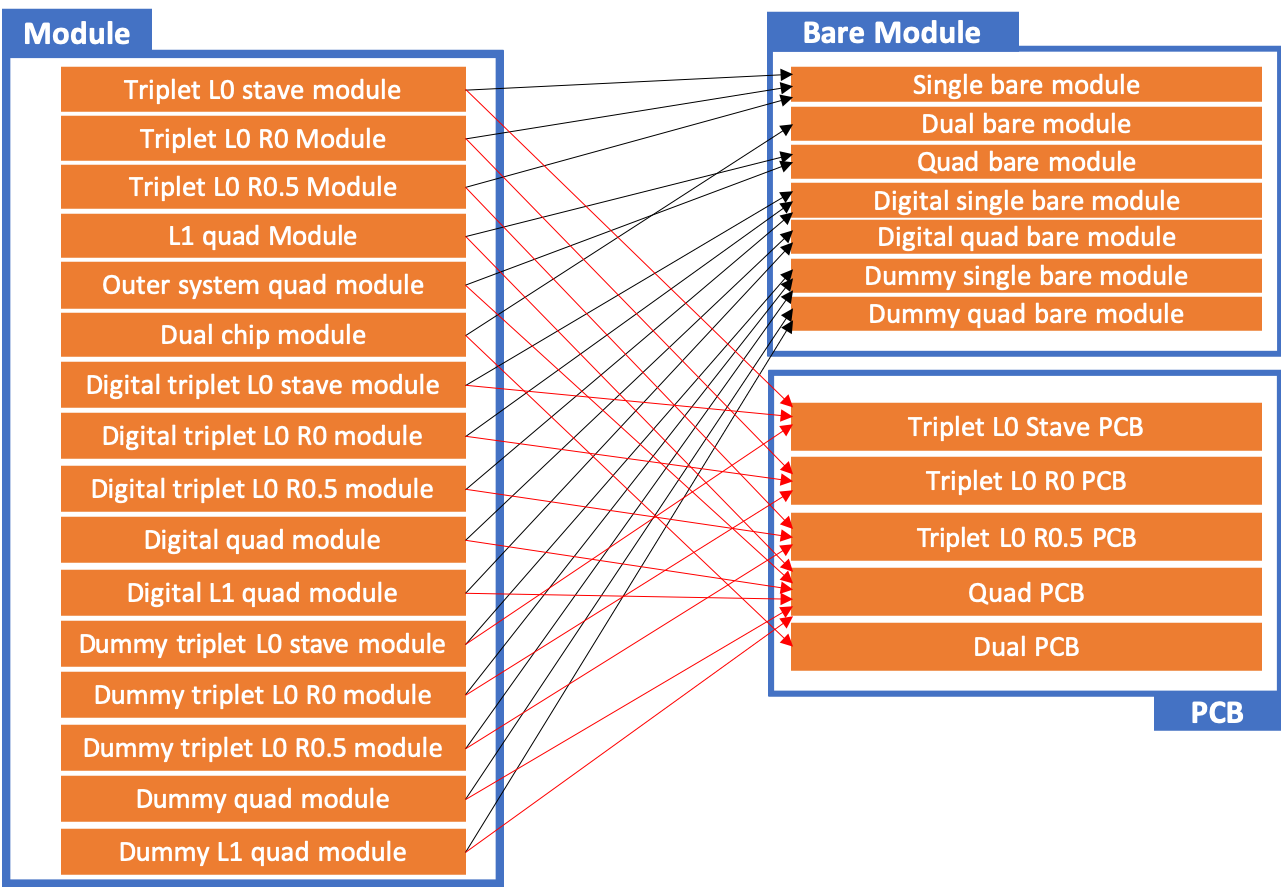
\includegraphics[width=12cm]{./pd_module_structure.png}
\caption[中央データベースにおけるモジュールの種類と構造]{中央データベースにおけるモジュールの種類と構造。中央データベースにモジュールを登録するときの情報として、モジュールの種類、構成部品を図のように実装した。図の左側に実装したモジュールの種類を示しており、Triplet、Quadというように、モジュールの種類ごとに登録できるシステムとなっている。また矢印は構成部品を指しており、各モジュールは対応するBare Module(ベアモジュール)とPCB(フレキシブル基板)を持つ。DBの中でモジュールと構成部品の紐付けも同時に行うことができる。}
\label{pd_module_structure}
\end{figure}

\begin{figure}[bpt]\centering
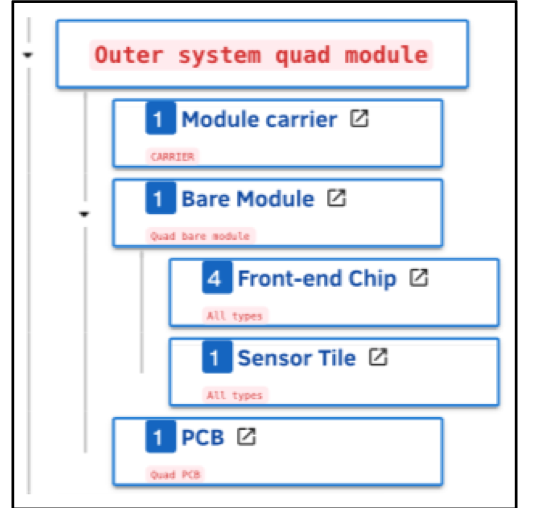
\includegraphics[width=6cm]{./example_module_structure.png}
\caption[中央データベース内におけるモジュール構造の一例(Quadモジュール)]{中央データベース内におけるモジュール構造の一例(Quadモジュール)。例としてOuter system quad moduleの中央データベース内の構造を示している。この種類では構成要素としてそれぞれ対応する種類のModule carrier、Bare Module、PCBを持つことがわかる。さらにBare ModuleはFE chipを4、Sensorを1持つことが分かり、Quadモジュールの構造が正しく実装されていることが分かる。}
\label{example_module_structure}
\end{figure}

\begin{table}[btp]
\begin{center}
\caption[中央データベースにおける組み立て工程と付随するテスト項目]{中央データベースにおける組み立て工程と付随するテスト項目。モジュールの組み立て工程及び品質試験をアップロードするため、表のような構造を実装した。データベース内でこの表に沿った組み立て工程の登録、更新、試験結果のアップロードができるようになった。}
\label{pd_stage_structure}
  \scriptsize
  \begin{tabular}{|ll|} \hline
    組み立て項目 & 付随する組み立て情報及び品質試験項目 \\ \hline
    1. Bare to PCB assembly & Visual Inspection \\ 
                            & Metrology \\
                            & Mass measurement \\
                            & Glue information \\\hline
    2. Wirebonding          & Visual Inspection \\ 
                            & Wirebond information \\
                            & (Wirebond pull test)\\
                            & First power up\\
                            & Sensor IV\\
                            & SLDO VI\\
                            & Chip configuration\\
                            & Pixel failure test\\\hline

    3. Wirebond Protection  & Visual Inspection \\ 
                            & Potting information \\
                            & Sensor IV \\
                            & Register test\\
                            & Readout for basic electrical \\\hline

    4. Parylene Coating     & Visual Inspection \\ 
                            & Palylene information \\
                            & Mass measurement \\
                            & Sensor IV \\
                            & Register test\\
                            & Readout for basic electrical \\
                            & Bump bond quality \\\hline

    5. Thermal Cycling      & Visual Inspection \\ 
                            & Thermal cycling info \\
                            & Sensor IV \\
                            & Register test\\
                            & Readout for basic electrical \\
                            & Bump bond quality \\\hline

    6. Burn-in              & Visual Inspection \\ 
                            & Metrology \\
                            & Mass Measurement \\
                            & First power up\\
                            & Sensor IV\\
                            & SLDO VI\\
                            & Chip configuration\\
                            & Pixel failure test\\\hline

    7. Reception            & \\\hline 
  \end{tabular}
\end{center}
\end{table}


\clearpage
%%%%%%%%%%%%%%%%%%%%%%%%%%%%%%%%%%%%%%%%%%%%%%%%%%%
%%%%%%%%%%%%%%%%%%%%%%%%%%%%%%%%%%%%%%%%%%%%%%%%%%%
%%%%%%%%%%%%%%%%%%%%%%%%%%%%%%%%%%%%%%%%%%%%%%%%%%%

\subsection{データベース同期ツールの開発} \label{sec:interfacing_tool}
モジュール情報や品質試験結果の共有のために、中央データベースとローカルデータベースの間で同期が行われる必要がある。
これを行うツールを設計、開発を行った。

ツールの中では中央データベースが開発、提供している中央データベース通信用APIと、節\ref{sec:web_app}で述べたローカルのMongoDBと通信するAPIの2つを用いることで同期を行っている。

同期ツール処理のイメージを図\ref{interfacing_tools_system}に示す。

\begin{figure}[bpt]\centering
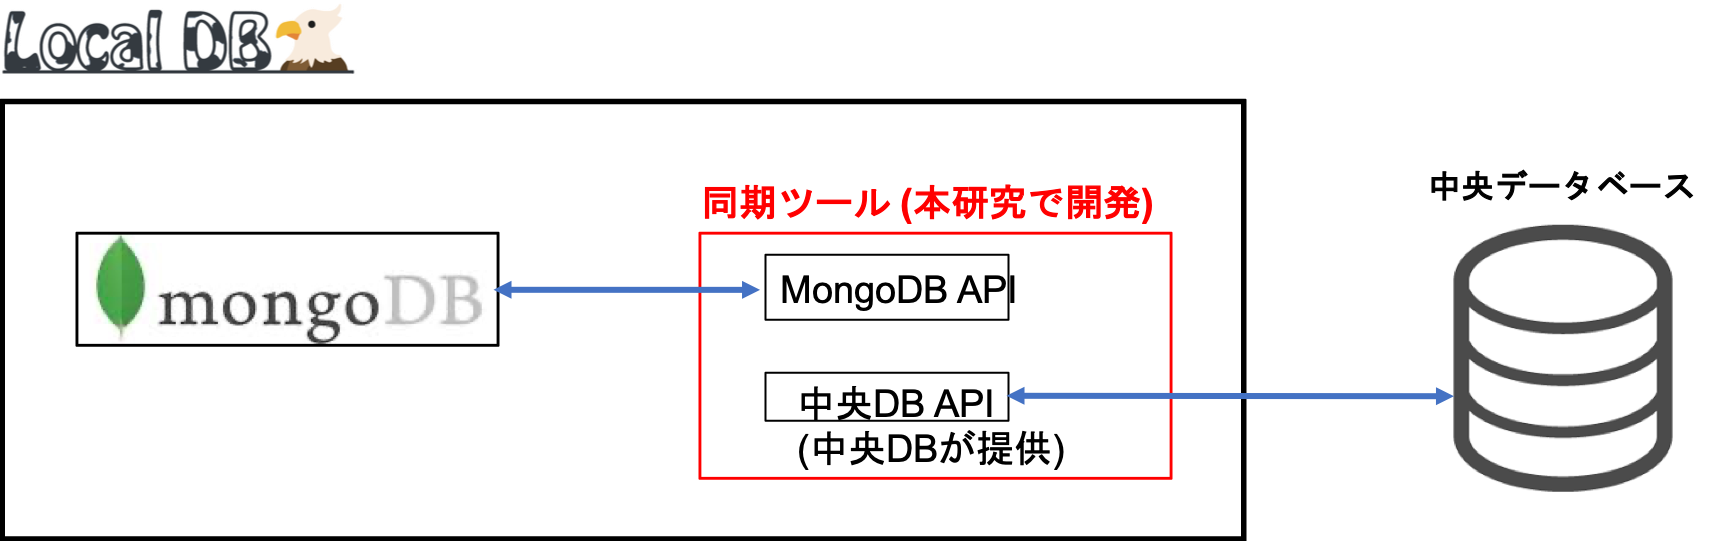
\includegraphics[width=13cm]{./interfacing_tools_system.png}
\caption[同期ツール処理のイメージ]{同期ツール処理のイメージ。本研究で開発を行っているのは図の赤線の領域に対応する同期ツールである。このツールはPythonを用いて開発しており、処理の中でローカルのMongoDBと通信するAPIと、中央データベースが開発、提供をしているAPIを用いることで、2つのデータベース間の同期を行っている。このとき、中央データベースとの通信はhttp通信で行われる。}
\label{interfacing_tools_system}
\end{figure}

特に本研究ではツールの枠組み設計に加えて、以下の機能を実装した。
\begin{itemize}
  \item モジュール及び構成するFEチップ情報のダウンロード機能.
  \item 読み出し試験結果のアップロード機能.
\end{itemize}

これらの機能のイメージを図\ref{interface_overview}に示す。
実装の詳細及び処理時間測定について8章で述べる。

\begin{figure}[bpt]\centering
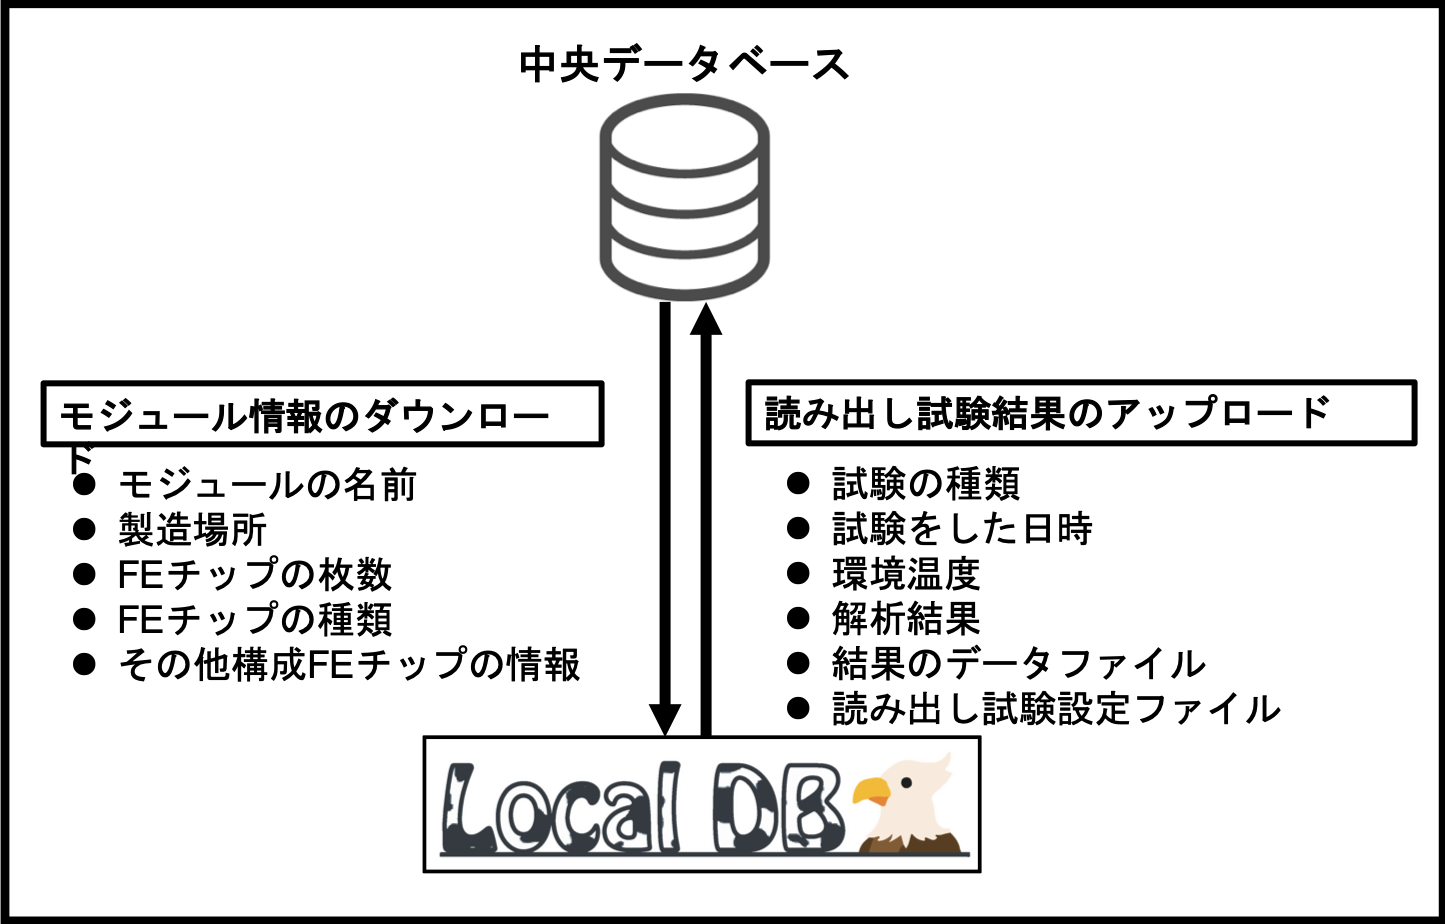
\includegraphics[width=11cm]{./interface_overview.png}
\caption[同期機能の概要]{同期機能の概要。本研究ではモジュール情報のダウンロードと読み出し試験結果のアップロード機能を実装した。図に示している情報を主に同期する機能となっている。}
\label{interface_overview}
\end{figure}

\clearpage
%%%%%%%%%%%%%%%%%%%%%%%%%%%%%%%%%%%%%%%%%%%%%%%%%%%
%%%%%%%%%%%%%%%%%%%%%%%%%%%%%%%%%%%%%%%%%%%%%%%%%%%
%%%%%%%%%%%%%%%%%%%%%%%%%%%%%%%%%%%%%%%%%%%%%%%%%%%

\subsection{ユーザ管理機能及び各種機能}

異常があった際に確認することを目的として、誰が試験を行ったかを記録することが必要である。
また、モジュールの登録や中央データベースとの同期など、データベースの機能使用を制限することも必要である。
これらを目的として、試験者及びデータベース使用者情報の管理機能を開発、実装した。
この詳細を以下で述べる。

\subsubsection{機能概要}
データベース権限の段階として、管理者、権限付きユーザ、一般ユーザの3段階を設けた。
各ユーザが使うことのできる機能を表\ref{user_functions_summary}に示す。

権限付きユーザの機能としてモジュール及び試験結果にコメント、タグをつける機能を実装した。使用したときの様子を図\ref{webapp_comment}、\ref{webapp_tag}に示す。

\subsubsection{ユーザ登録操作}
表\ref{user_functions_summary}において管理者と権限付ユーザの登録について説明する。

データベースシステム導入時に管理者のアカウントを作成する。
コマンドプロンプト上で開発したスクリプトを用いて実行することで管理者登録が行われる。この際ユーザ名とパスワードを入力する。

権限付ユーザについて、全ての品質試験者及びデータベースユーザ機能使用者は管理者によってユーザ登録される必要がある。
登録はウェブアプリケーションを用いて行い、以下の情報を入力する。
\begin{itemize}
  \item ユーザ名 
  \item 氏名
  \item 所属機関
  \item メールアドレス 
\end{itemize}

管理者が登録を完了すると、登録されたメールアドレスに登録完了メールと仮パスワードが届く。
このメールに従い、ウェブアプリケーション上でユーザがパスワード登録を完了する。

このようにメール機能を用いることでパスワード漏洩の防止、管理者操作の削減を目的としている。

\clearpage
%%%%%%%%%%%%%%%%%%%%%%%%%%%%%%%%%%%%%%%%%%%%%%%%%%%
%%%%%%%%%%%%%%%%%%%%%%%%%%%%%%%%%%%%%%%%%%%%%%%%%%%
%%%%%%%%%%%%%%%%%%%%%%%%%%%%%%%%%%%%%%%%%%%%%%%%%%%
\begin{table}[btp]
\begin{center}
\caption[ローカルデータベースユーザ権限及び使用機能一覧]{ローカルデータベースユーザ権限及び使用機能一覧。ローカルデータシステムにおけるユーザとして、管理者、権限付きユーザ、一般ユーザの3つを設けた。全てのユーザがウェブアプリケーションの閲覧をすることができる。管理者、権限付きユーザにはデータベース読み書き権限とウェブアプリケーションログイン権限が与えられ、試験結果のアップロード、アプリケーション上のユーザ機能の実行ができる。また管理者は権限付きユーザを登録することができる。}
\label{user_functions_summary}
  \small
  \begin{tabular}{|lll|} \hline
    ユーザ       & 付加される権限                               & 使用できる機能 \\ \hline
    管理者       & ユーザ管理権限                     & 権限付きユーザ登録機能\\ 
                 & データベース読み書き権限           & \\ 
                 & ウェブアプリケーションログイン権限 & \\ \hline
    権限付ユーザ & データベース読み書き権限           & 試験結果のアップロード\\ 
                 & ウェブアプリケーションログイン権限 & 中央データベースとの同期機能\\ 
                 &                                    & その他ウェブアプリケーションの機能(コメント、タグ)\\ \hline
    一般ユーザ   &                                    & モジュール情報及び試験結果の閲覧 \\ \hline
  \end{tabular}
\end{center}
\end{table}

\begin{figure}[btp]\centering
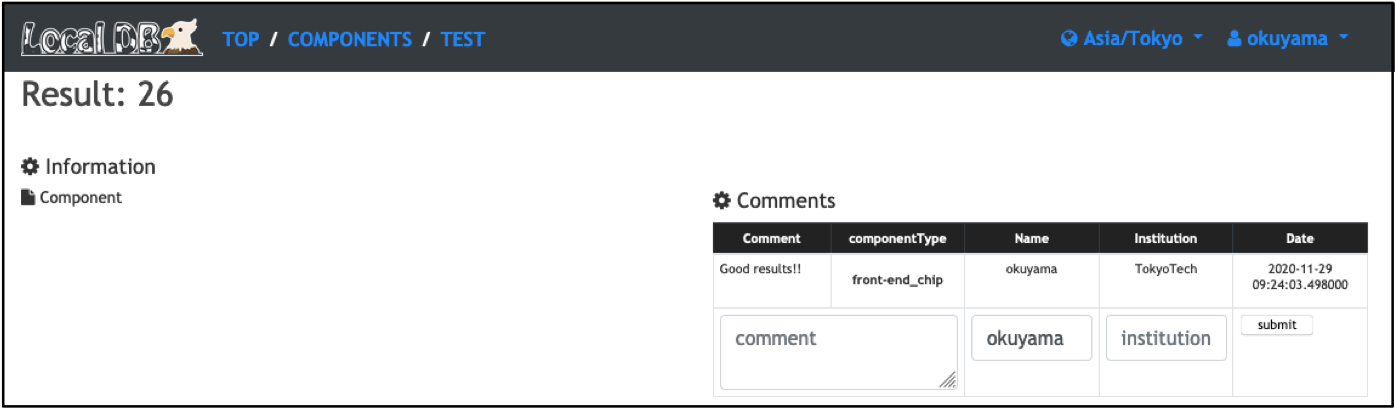
\includegraphics[width=12cm]{./viewer_comment.png}
\caption[ウェブアプリケーションにおけるコメント機能]{ウェブアプリケーションにおけるコメント機能。権限付きユーザ及び管理者はモジュールや試験結果に対してコメントをすることができる。図のようにページの右側にコメント欄があり、コメントをテキスト形式で記述することができる。}
\label{webapp_comment}
\end{figure}

\begin{figure}[bpt]\centering
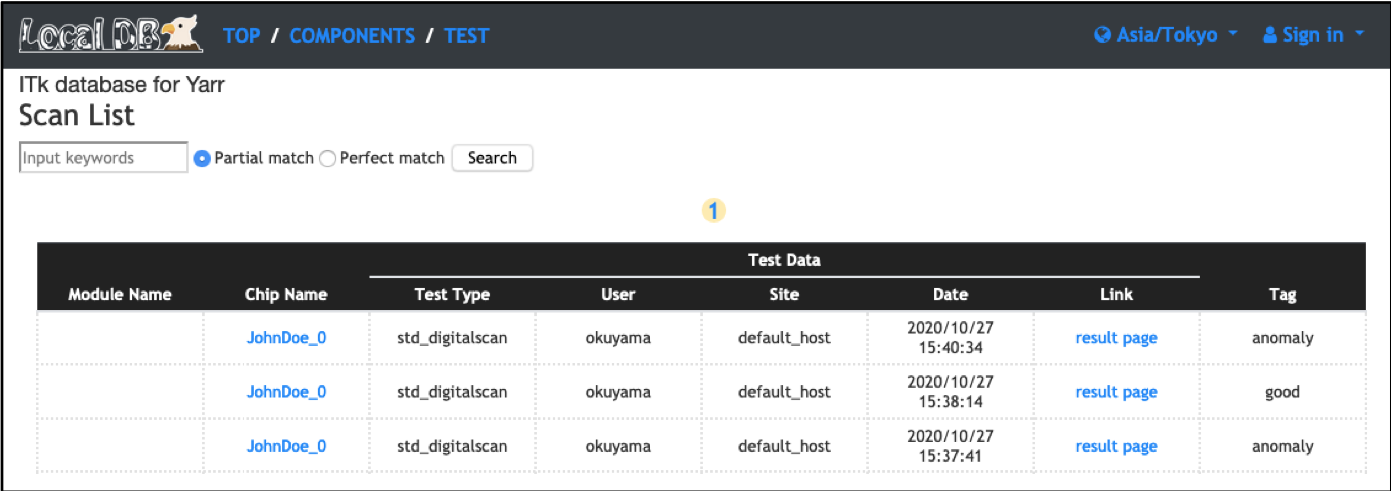
\includegraphics[width=12cm]{./viewer_tag.png}
\caption[ウェブアプリケーションにおけるタグ機能]{ウェブアプリケーションにおけるタグ機能。権限付きユーザ及び管理者はモジュールや試験結果に対してタグをつけることができる。図は試験結果の一覧ページであり、図の表において一番右の列がつけられたタグを示しており、図ではanomalyやgoodといったタグが付けられていることが分かる。}
\label{webapp_tag}
\end{figure}

\clearpage
%%%%%%%%%%%%%%%%%%%%%%%%%%%%%%%%%%%%%%%%%%%%%%%%%%%
%%%%%%%%%%%%%%%%%%%%%%%%%%%%%%%%%%%%%%%%%%%%%%%%%%%
%%%%%%%%%%%%%%%%%%%%%%%%%%%%%%%%%%%%%%%%%%%%%%%%%%%

\subsubsection{機能の仕組み}
ユーザ登録の際には内部で以下の2つの処理が行われるように実装した。

\begin{enumerate}
  \item MongoDBアカウントの作成、読み書き権限の付与.
  \item ウェブアプリケーションで用いるユーザ情報ドキュメントの作成.
\end{enumerate}

1の処理を行う理由は、登録ユーザが試験結果をMongoDBにアップロードできるようにするためである。
2の情報は、ウェブアプリケーション内でのログイン判断、ユーザの情報保持に使う。
この情報は表\ref{localdb_structure}のviewer.userに保存される。
2つの処理について、実際に保存されるドキュメントの例をコード\ref{user_doc_1}、\ref{user_doc_2}以下に示す。

\begin{lstlisting}[basicstyle=\scriptsize,caption=MongoDBアカウント情報を持つドキュメントの例。リスト中の"roles"より、localdbとlocaldbtoolsの読み書き権限が付加されていることが分かる。,label=user_doc_1]
{
	"_id" : "localdb.hokuyama",
	"userId" : UUID("fee321eb-83b8-434a-a4a0-fff638b5db36"),
	"user" : "hokuyama",
	"db" : "localdb",
	"credentials" : {
    ...
	},
	"roles" : [
		{
			"role" : "readWrite",
			"db" : "localdb"
		},
		{
			"role" : "readWrite",
			"db" : "localdbtools"
		}
	]
}
\end{lstlisting}

\begin{lstlisting}[basicstyle=\scriptsize,caption=ウェブアプリケーションで扱うユーザ情報を持つドキュメントの例。リスト\ref{user_doc_1}で示したものとは別に、ウェブアプリケーション内でユーザ情報を扱うためにこのドキュメントを保持する必要がある。ウェブにおいてログインはこのドキュメントの存在確認をもってなされる。パスワードはhash化して保存している。,label=user_doc_2]
{
	"_id" : ObjectId("5f0bbe84ef87af2628865de7"),
	"sys" : {
		"rev" : 0,
		"cts" : ISODate("2020-07-13T10:53:07.943Z"),
		"mts" : ISODate("2020-07-13T10:53:07.943Z")
	},
	"username" : "hokuyama",
	"name" : "Hiroki Okuyama",
	"auth" : "readWrite",
	"institution" : "Tokyo Institute of Technology",
	"Email" : "okuyama@hep.phys.titech.ac.jp",
	"password" : "5f4dcc3b5aa765d61d8327deb882cf99"
}
\end{lstlisting}

\clearpage
%%%%%%%%%%%%%%%%%%%%%%%%%%%%%%%%%%%%%%%%%%%%%%%%%%%%%%%
%%%%%%%%%%%%%%%%%%%%%%%%%%%%%%%%%%%%%%%%%%%%%%%%%%%
%%%%%%%%%%%%%%%%%%%%%%%%%%%%%%%%%%%%%%%%%%%%%%%%%%%%%%%
\newpage
\subsection{品質試験結果の登録と組み立て工程の自動更新}
ローカルデータベースへアップロードした品質試験結果の中から、本結果として中央データベースへ同期する結果を選択する必要ある。
これは不必要な結果を同期せず、中央データベースを簡潔に保つ目的がある。
この結果選択機能を開発した。
品質試験は各モジュール、各組み立て工程に対して行うものであるため、結果選択も同様に工程毎に行うことを想定している。
結果選択後、データベースにおける組み立て工程は次のものへ自動的に更新する機能となっている。

\subsubsection{概要}
あるモジュール、組み立て工程に対して結果を選択する様子を図\ref{webapp_sign_off}に示す。組み立て工程も自動更新されていることがわかる。

\subsubsection{仕組み}
コード\ref{qc_status}、\ref{qc_module_status}のようなドキュメントを作成、保存する。
コード\ref{qc_status}は全てのモジュールに対して共通のドキュメントであり、組み立て工程と各工程における品質試験項目を記録する。
これらの情報は中央データベースから取得する。
この情報を参照することでローカルデータベース内部で組み立て工程の管理が可能となる。

コード\ref{qc_module_status}は各モジュールに対して1つ存在し、以下のような情報を保持する。
\begin{itemize}
  \item モジュールの現組み立て工程.
  \item 各工程における選択された品質試験結果のID.
\end{itemize}


\begin{lstlisting}[basicstyle=\scriptsize,caption=組み立て工程及び品質試験一覧情報のドキュメント。このようなドキュメントを作成、保持しておくことで組み立て工程及び品質試験の情報を扱う。ローカルデータベース内に1つこのドキュメントを保持し、品質試験結果選択、組み立て工程の更新時にこのドキュメントを参照する。このドキュメントは中央データベースより取得して作成する。,label=qc_status]
{
	"_id" : ObjectId("5fc89aa232d56b29091fd64d"),
	"sys" : {
		"mts" : ISODate("2020-12-03T07:58:26.310Z"),
		"cts" : ISODate("2020-12-03T07:58:26.310Z"),
		"rev" : 0
	},
	"dbVersion" : 1.01,
	"proddbVersion" : 1.01,
	"stage_flow" : [
		"MODULETOPCB",
		"MODULEWIREBONDING",
		"MODULEWIREBONDPROTECTION",
		"MODULEPARYLENECOATING",
		"MODULETHERMALCYCLING",
		"MODULEBURNIN",
		"MODULERECEPTION"
	],
	"stage_test" : {
		"MODULETOPCB" : [
			"OPTICAL",
			"GLUE_MODULE_FLEX_ATTACH",
			"MASS",
			"METROLOGY"
		],
		"MODULEWIREBONDING" : [
			"WIREBONDING",
			"OPTICAL",
			"SENSOR_IV",
			"PIXEL_FAILURE_TEST",
			"SLDO_VI",
			"WIREBOND",
			"CHIP_CONFIGURATION"
		],
		"MODULEWIREBONDPROTECTION" : [
			"OPTICAL",
			"POTTING",
			"MASS",
			"READOUT_IN_BASIC_ELECTRICAL_TEST",
			"SENSOR_IV",
			"REGISTER_TEST"
		],
    ...
	},
...
}
\end{lstlisting}

\begin{lstlisting}[basicstyle=\scriptsize,caption=モジュールの組み立て工程及び品質試験結果管理のためのドキュメント例。各モジュールにおいて現在の組み立て工程及び選択された品質試験結果がこのドキュメントに保存される。ドキュメント内の"currentStage"に現工程を保持する。また選択した試験結果のIDを"QC$\_$results"に、組み立て工程ごとに保持する。,label=qc_module_status]
{
	"_id" : ObjectId("5fc4be4c12a45922a91b0e75"),
	"sys" : {
		"mts" : ISODate("2020-11-30T09:41:32.411Z"),
		"cts" : ISODate("2020-11-30T09:41:32.411Z"),
		"rev" : 0
	},
	"dbVersion" : 1.01,
	"proddbVersion" : 1.01,
	"component" : "5fa79114e615fa000a1a5976",
	"currentStage" : "MODULEWIREBONDPROTECTION",
	"latestSyncedStage" : "MODULEWIREBONDING",
	"status" : "created",
	"rework_stage" : [ ],
	"QC_results" : {
		"MODULETOPCB" : {
			"OPTICAL" : "5fc4c2cfb6c93d451e2c9ac1",
			"GLUE_MODULE_FLEX_ATTACH" : "-1",
			"MASS" : "5fc4c2da27766dc6e89c024f",
			"METROLOGY" : "5fc4c2eaf1f19d9cb5859f00"
		},
		"MODULEWIREBONDING" : {
			"WIREBONDING" : "-1",
			"OPTICAL" : "5fc4c4c8b7d0c86912b4958f",
			"SENSOR_IV" : "5fc4c59e9e283a57ccaa1088",
			"PIXEL_FAILURE_TEST" : "5fca342f6e9f1f5eafedfb92",
			"SLDO_VI" : "-1",
			"WIREBOND" : "-1",
			"CHIP_CONFIGURATION" : "-1"
		},
		"MODULEWIREBONDPROTECTION" : {
			"OPTICAL" : "-1",
			"POTTING" : "-1",
			"MASS" : "-1",
			"READOUT_IN_BASIC_ELECTRICAL_TEST" : "-1",
			"SENSOR_IV" : "-1",
			"REGISTER_TEST" : "-1"
		},
    ...
	}
}
\end{lstlisting}

\begin{figure}[bpt]\centering
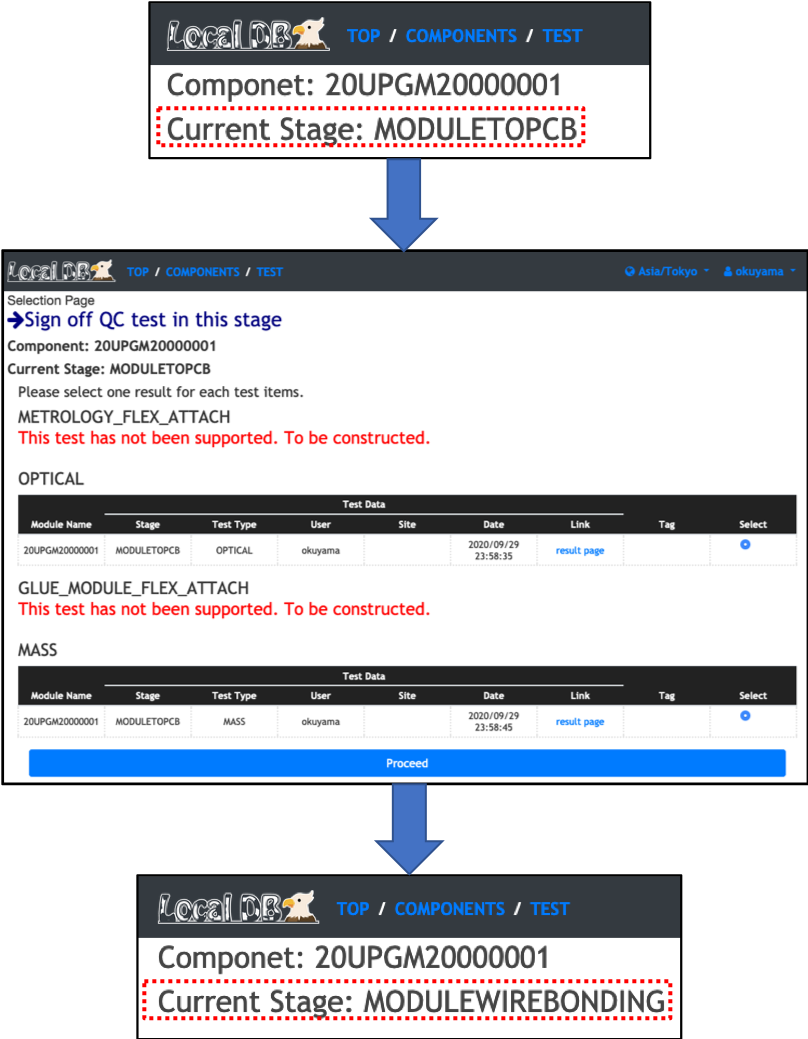
\includegraphics[width=14cm]{./webapp_sign_off.png}
\caption[結果選択画面及び組み立て工程表示の例]{結果選択画面及び組み立て工程表示の例。図の上部で組み立て工程が"MODULETOPCB"である。図の中部において品質試験結果選択処理を行なっており、この図では"OPTICAL"と"MASS"の結果を選択している。この時、ローカルデータベース内部では選択された結果にタグ付けがなされる。これらの結果は中央データベースと同期される。また結果選択後は組み立て工程が自動的に更新される。図の下部では"MODULEWIREBONDING"になっていることが分かる。}
\label{webapp_sign_off}
\end{figure}

\clearpage
%%%%%%%%%%%%%%%%%%%%%%%%%%%%%%%%%%%%%%%%%%%%%%%%%%%%%%%
%%%%%%%%%%%%%%%%%%%%%%%%%%%%%%%%%%%%%%%%%%%%%%%%%%%%%%%

\newpage
\subsection{読み出し試験結果におけるピクセル解析ツール}
節\ref{sec:pixel_analysis}で述べたように、読み出し試験ではピクセル解析を行う。
これを円滑に行うために、ピクセル解析ツールを開発した。また開発した解析ツールをローカルデータベースシステムに組み込んだ。
このツールについての詳細を以下に示す。

\subsubsection{概要}
YARRで読み出し試験を行った場合、結果ファイル及びディレクトリは各試験項目ごとにわかれて生成される。
また各結果ファイルにはモジュール上の全ピクセル結果がJSONの形で保存されている。

一方、ピクセル解析において、いくつかの試験結果を統一的に扱い、各ピクセルごとに解析を行う必要がある。
そこで、開発した解析ツールでは複数の結果ファイルを1つに統合し、ピクセルごとの解析処理を単純化する役割を担っている。
開発にはPythonとC++を用いた。またCERNが提供している解析フレームワークであるROOT\cite{4-5}を使用し、いくつかの試験データの統一ファイルとして、ROOT内部機能であるTreeを使用した。
このファイル統合処理のイメージを図\ref{analysis_tool_motivation}に示す。

\begin{figure}[bpt]\centering
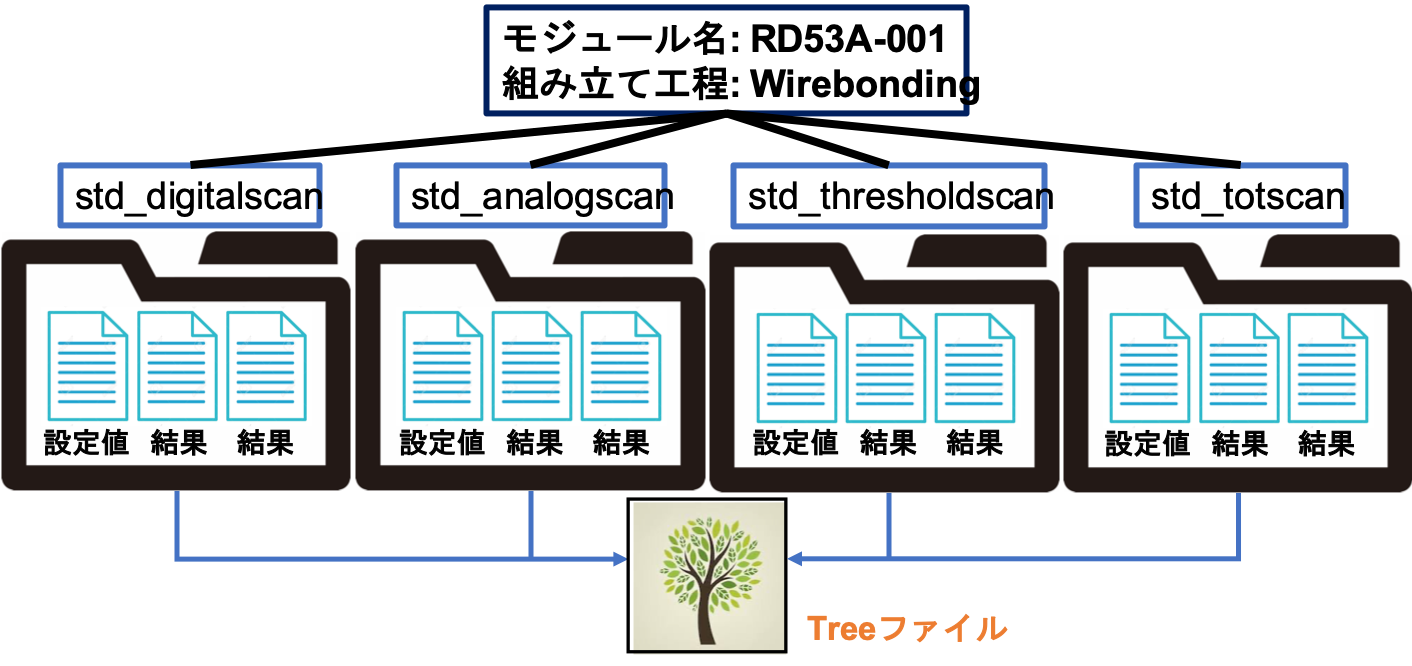
\includegraphics[width=12cm]{./analysis_tool_motivation.png}
\caption[ピクセル解析ツールにおけるファイル統合処理のイメージ]{ピクセル解析ツールにおけるファイル統合処理のイメージ。YARRの出力ファイル及びディレクトリは\texttt{std$\_$digitalscan}や\texttt{std$\_$thresholdscan}というように読み出し項目ごとである。ピクセル解析ツールでは、図のようにあるモジュールに関連する結果ファイルを統合し、ピクセルごとに行う解析処理を簡易化する狙いがある。}
\label{analysis_tool_motivation}
\end{figure}

実際に作ったTreeファイルと、データ構造のイメージを図\ref{analysis_tool_tree}に示す。

\begin{figure}[bpt]
  \begin{minipage}{0.4\hsize}
    \begin{center}
    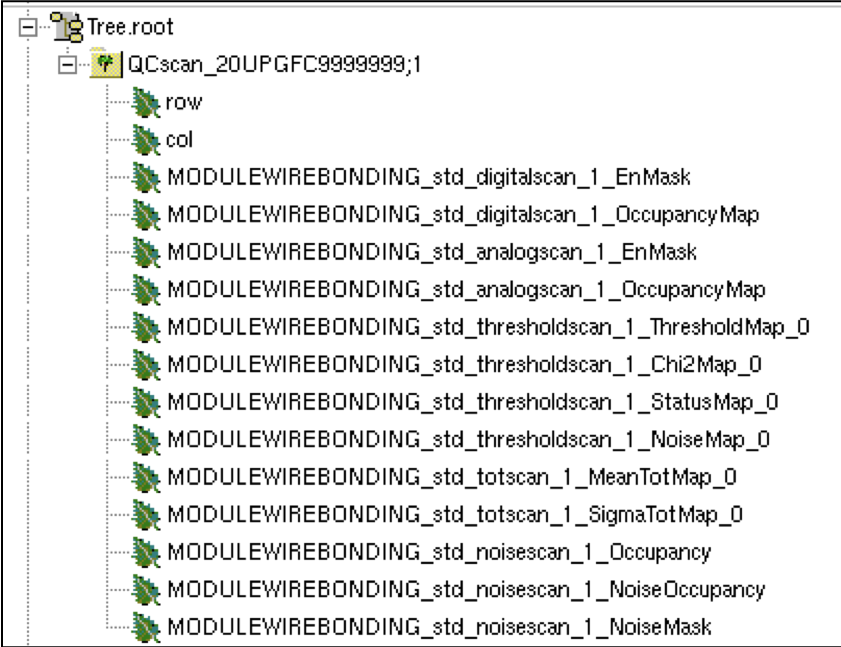
\includegraphics[width=6cm]{./analysis_tool_tree_file.png}
    \end{center}
  \end{minipage}
  \begin{minipage}{0.4\hsize}
    \begin{center}
    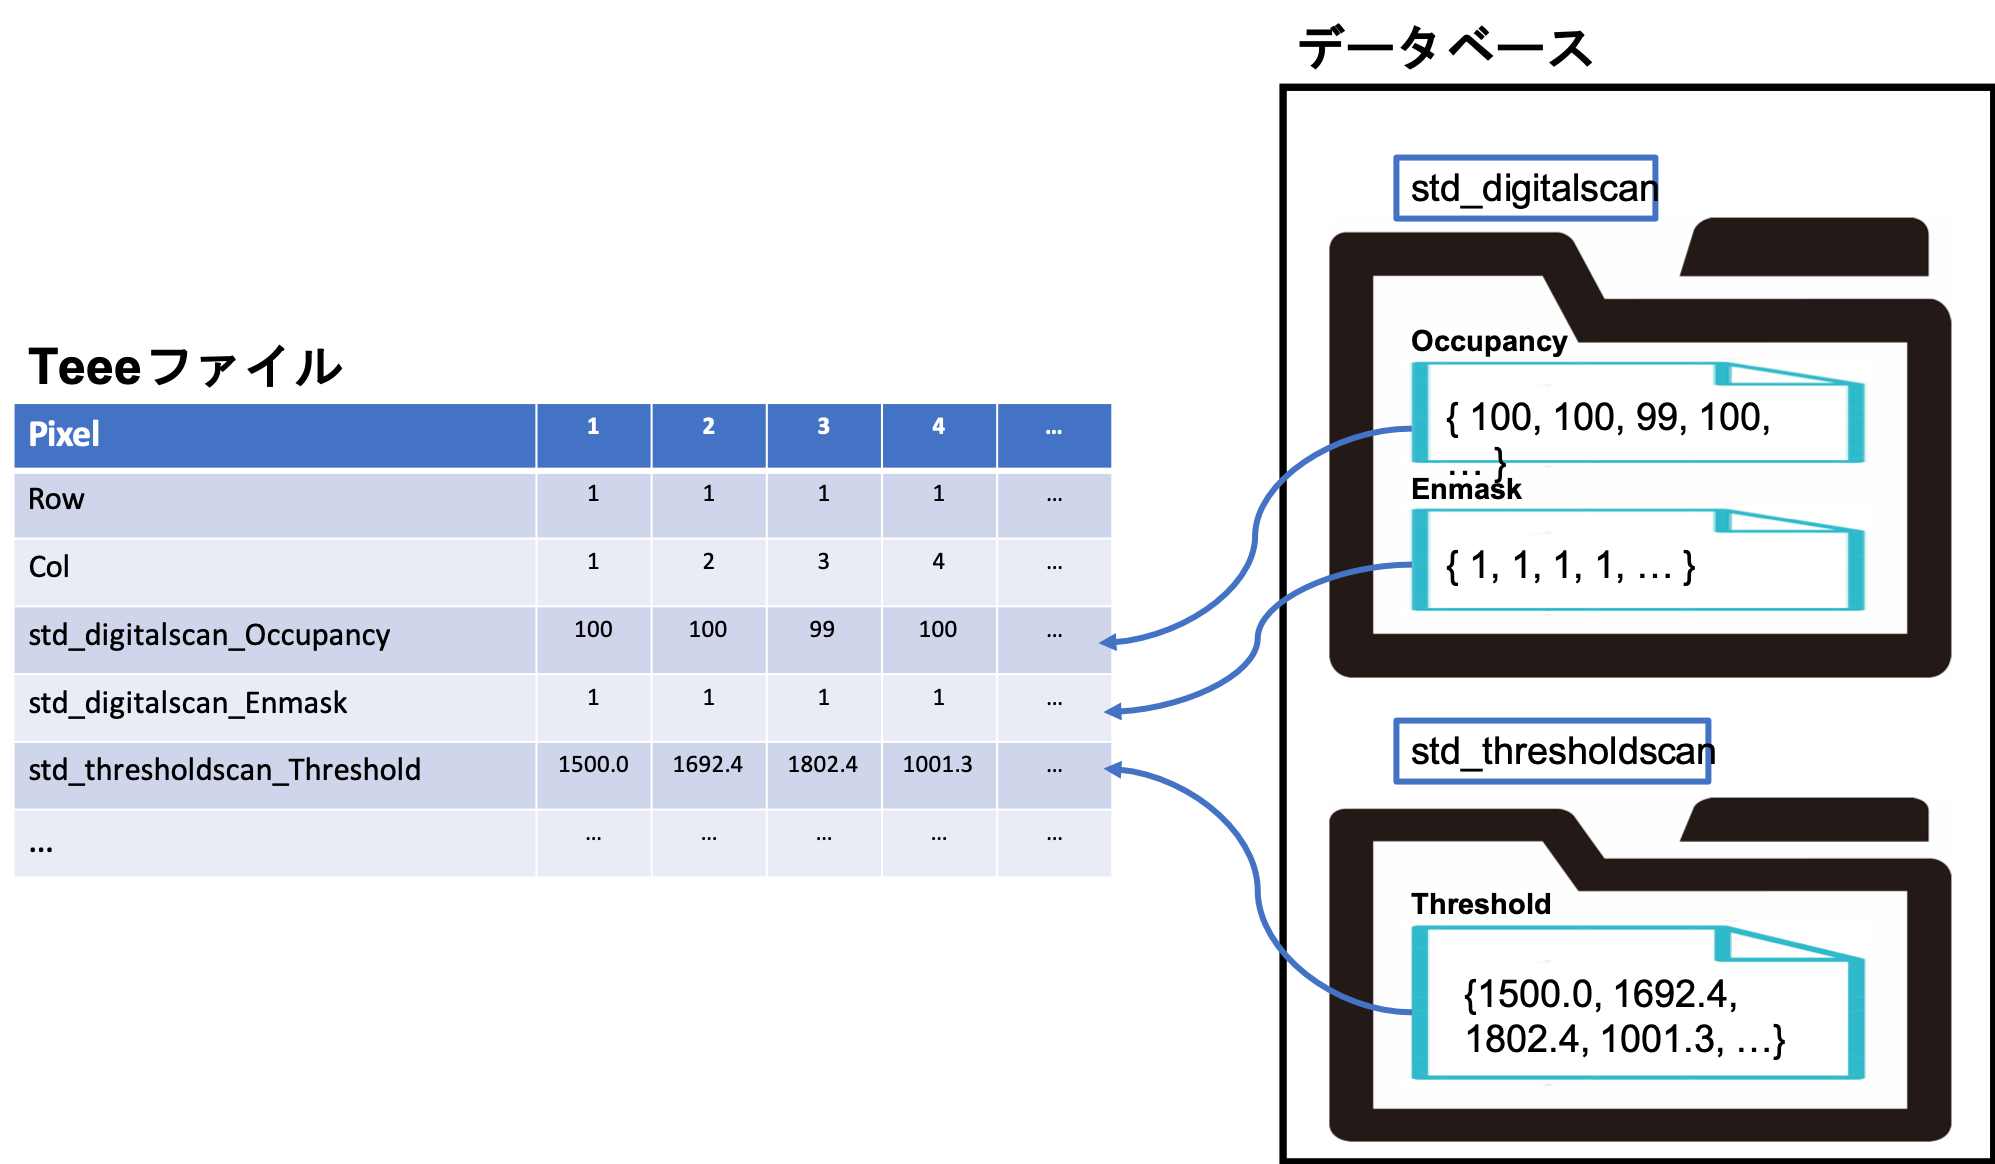
\includegraphics[width=8cm]{./analysis_tool_tree_image.png}
    \end{center}
  \end{minipage}
  \caption[Treeファイルとそのデータ保持のイメージ]{Treeファイルとそのデータ保持のイメージ。実際にこのツールを用いて作ったTreeファイルの内部構造の様子(左)とそのデータ保持のイメージ(右図)を示す。Treeファイルでは、右図のように1つの表に試験結果をまとめている。各行が\texttt{std$\_$digitalscan}といった各読み出し項目に対応し、各列が1ピクセルに対応する。モジュール上の行列(Row、Col)の番号を表の上部に持っておくことで、モジュール上におけるピクセルの位置情報を保持する。}
  \label{analysis_tool_tree}
\end{figure}

\subsubsection{ツールの内部構造と処理の流れ}
開発したツールは、主に以下で説明する3つの実行ファイルで構成される。それぞれの役割について説明する。

\begin{description}
  \item[getData.py (Python)]\mbox{}\\ 
    データベースから対象となるデータファイルを取得、キャッシュファイルとしてサーバー上の一時ディレクトリに保存.
  \item[makeTree (C++)]\mbox{}\\ 
    getData.pyを用いて生成されたキャッシュファイルを読み込み、Treeファイルを作成.
  \item[analysis (C++)]\mbox{}\\ 
  作成したTreeファイルを読み込みピクセル解析を実行、結果値やプロットを出力.
\end{description}

処理の流れのイメージを図\ref{analysis_tool_flow}に示す。
データベースとの通信に関してはMongoDBや現システムとの親和性を考慮し、Pythonを使用した。
Treeファイル作成やその後の解析処理のスクリプトは、ROOTを使用する観点からC++を使用した。
またピクセル解析以外の解析に対しても適応可能とするため、Tree作成部と解析処理部のファイルは分割した。

\begin{figure}[bpt]\centering
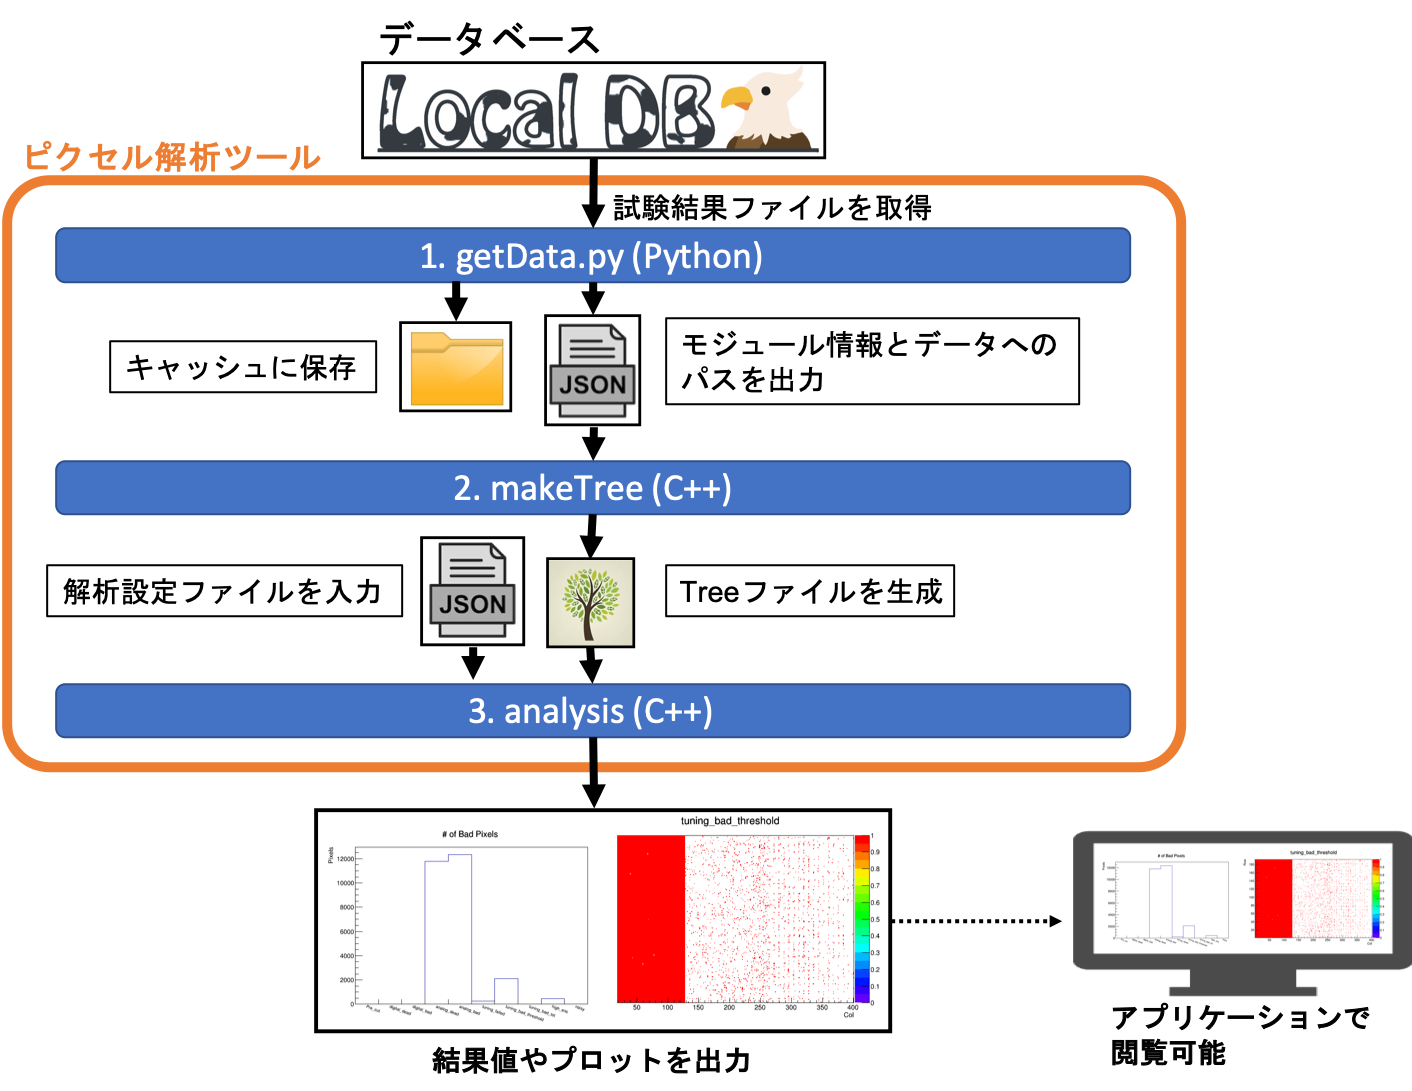
\includegraphics[width=10cm]{./analysis_tool_flow.png}
\caption[ピクセル解析ツールの処理の流れ]{ピクセル解析ツールの処理の流れ。ピクセル解析ツールは、図のように3つの実行ファイルにより構成される。getData.py(Python)にてデータベースから結果の取得を行い、makeTree(C++)にてTreeファイルの作成、analysis(C++)にてピクセル解析及び結果のプロットが出力される。}
\label{analysis_tool_flow}
\end{figure}

\clearpage
%%%%%%%%%%%%%%%%%%%%%%%%%%%%%%%%%%%%%%%%%%%%%%%%%%%%%%%
%%%%%%%%%%%%%%%%%%%%%%%%%%%%%%%%%%%%%%%%%%%%%%%%%%%%%%%
%%%%%%%%%%%%%%%%%%%%%%%%%%%%%%%%%%%%%%%%%%%%%%%%%%%
\subsection{読み出し試験結果の検索機能}
登録モジュールや品質試験結果の一覧ページに検索機能を実装した。
確認したいモジュール情報や試験結果を迅速に取得し、閲覧できることを目的としている。検索機能を使用している様子を図\ref{webapp_search_function}に示す。

キーワードを入力し、検索することができる仕組みとなっていて、一般的なウェブページの検索エンジンのように扱うことができる。
生産に向けて、検索にかかる処理時間測定を行った。検索機能実装方法の詳細と処理時間についての詳細は、6章で述べる。
現在は単一キーワード検索の他に、以下の機能を実装している。
\begin{itemize}
  \item 完全一致、部分一致検索.
  \item AND、OR検索.
\end{itemize}

\begin{figure}[bpt]\centering
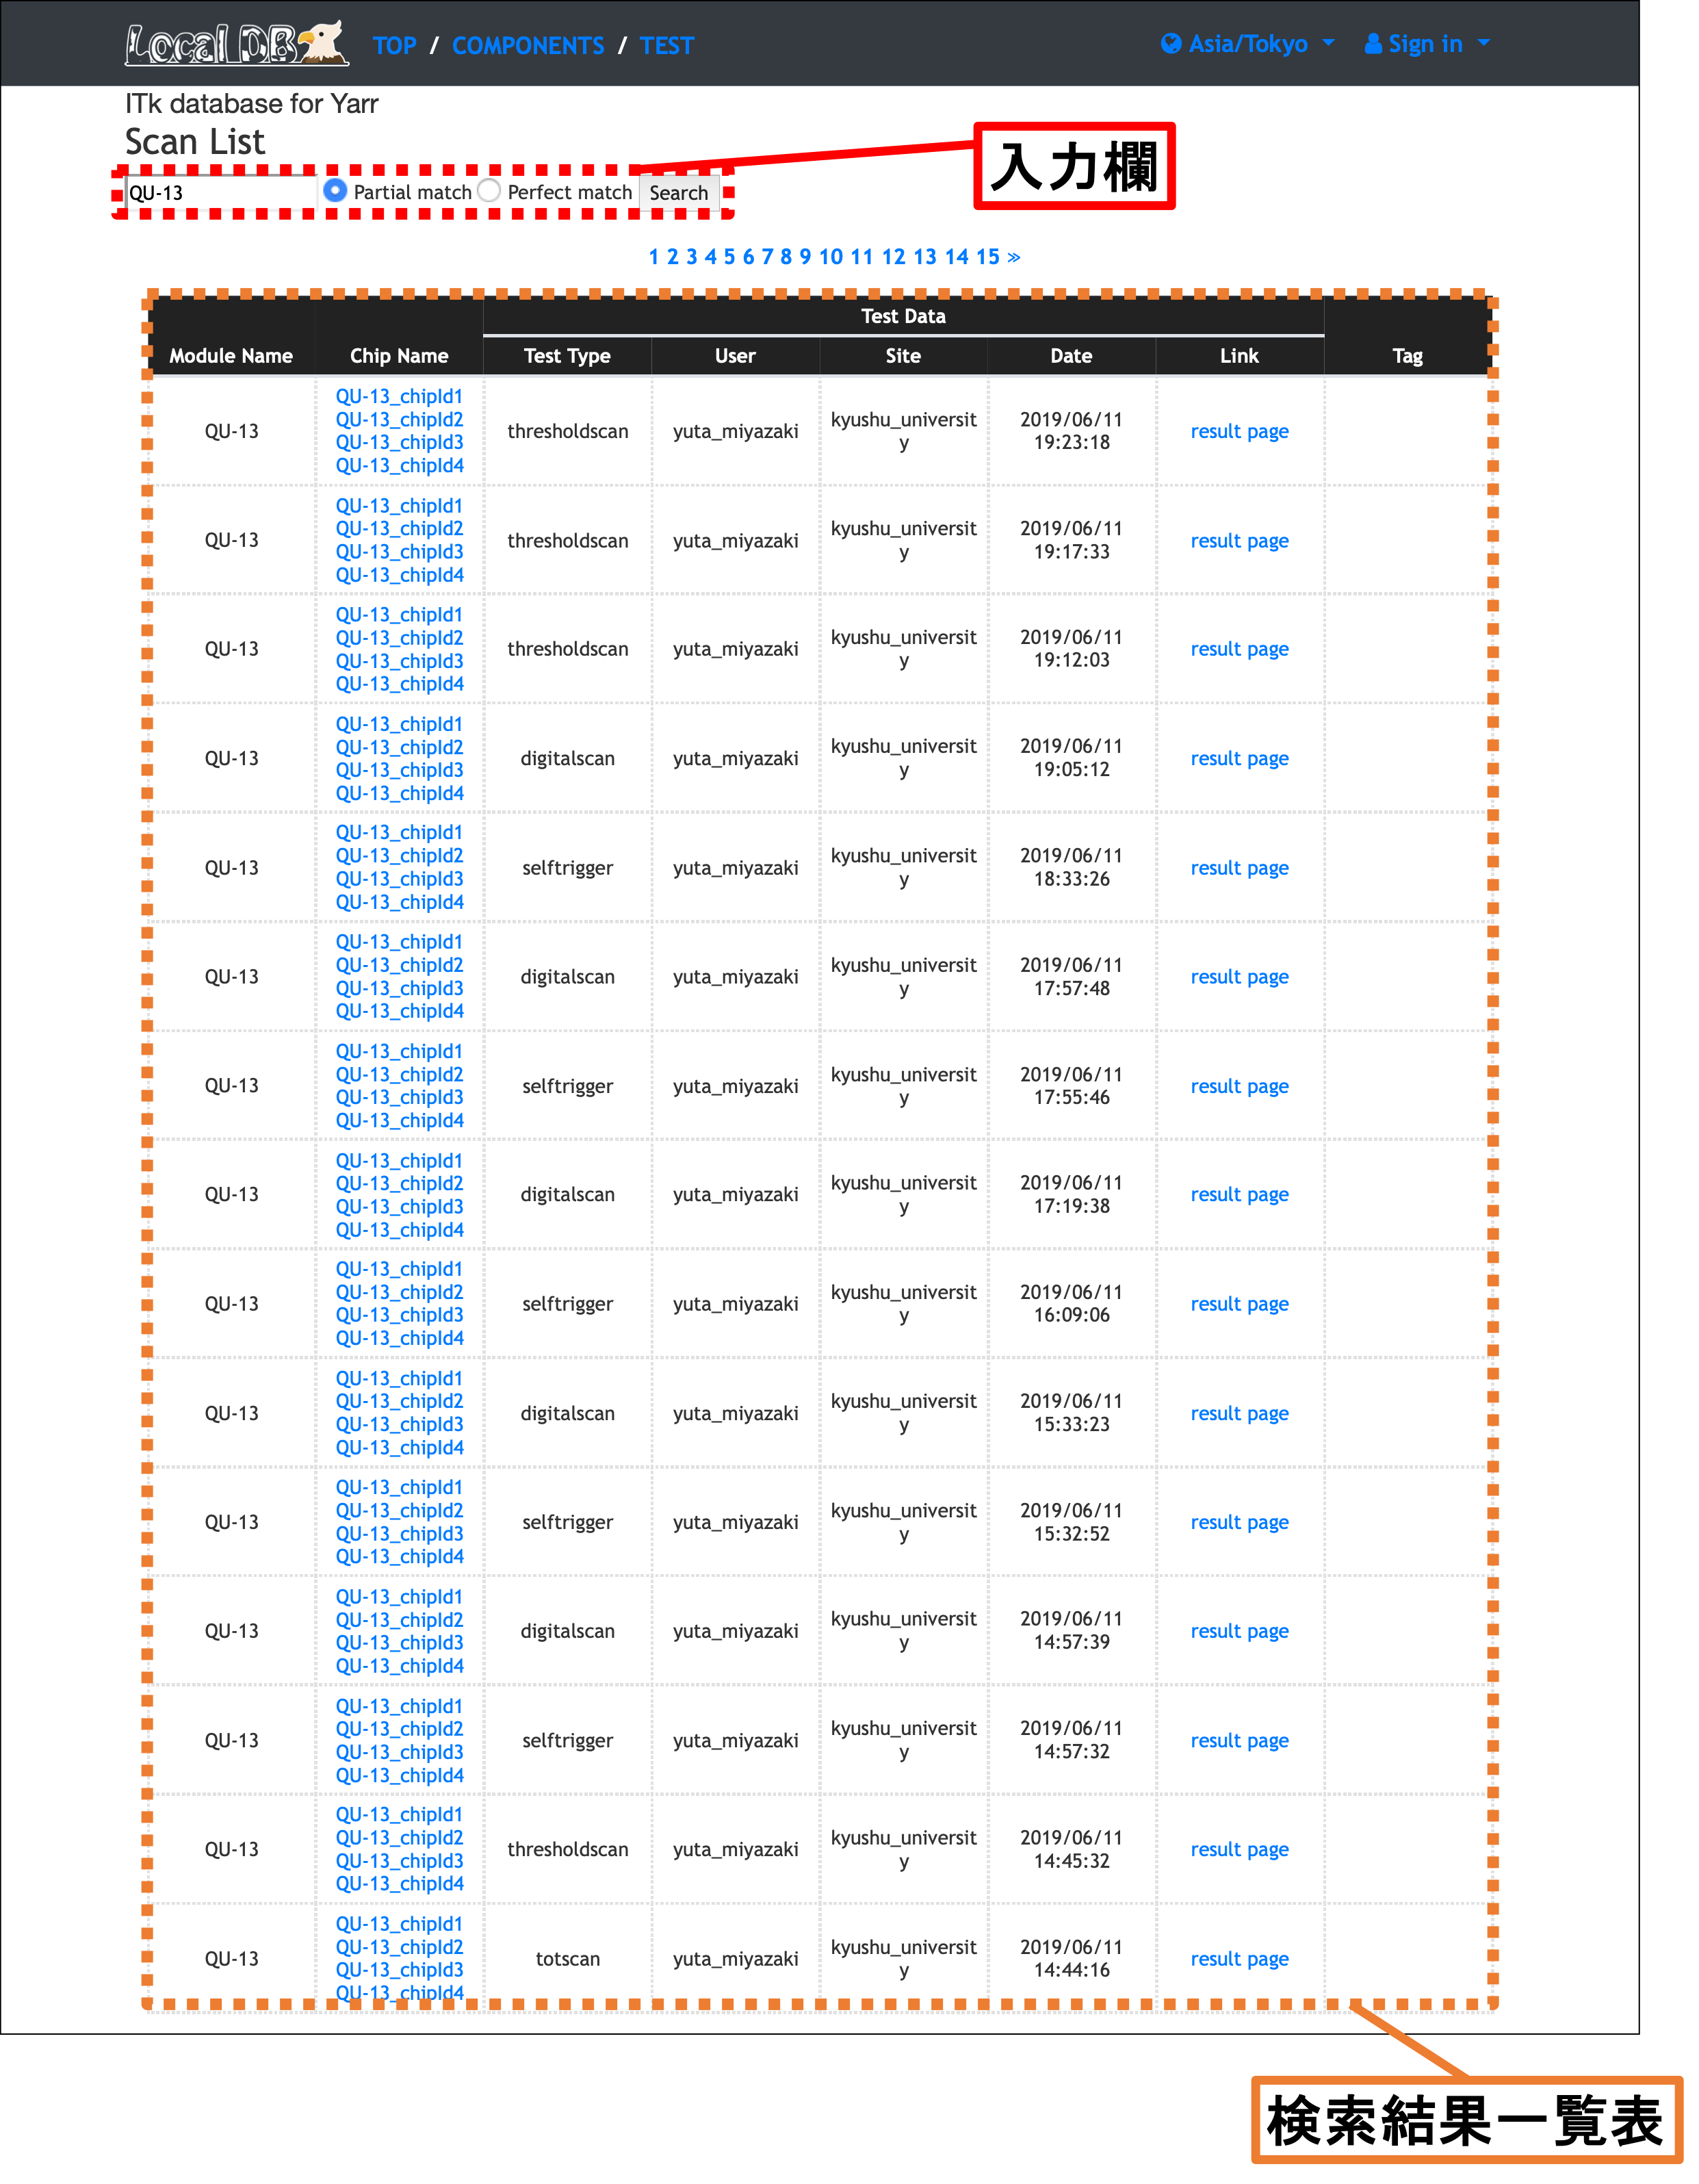
\includegraphics[width=10.5cm]{./webapp_search_function.png}
\caption[ウェブアプリケーションにおける検索機能の様子]{ウェブアプリケーションにおける検索機能の様子。図は検索結果一覧表示のページである。図の上部に入力欄があり(赤破線)、ここにキーワードを入力し検索を実行する。図の例で``QU-13"と入力しており、検索結果にはモジュール名「QU-13」の試験結果が一覧表示されていることが分かる。}
\label{webapp_search_function}
\end{figure}


\clearpage
%%%%%%%%%%%%%%%%%%%%%%%%%%%%%%%%%%%%%%%%%%%%%%%%%%%%%%%
%%%%%%%%%%%%%%%%%%%%%%%%%%%%%%%%%%%%%%%%%%%%%%%%%%%%%%%
%%%%%%%%%%%%%%%%%%%%%%%%%%%%%%%%%%%%%%%%%%%%%%%%%%%%%%%
\subsection{量産時におけるデータベース操作の流れの確立}
量産時におけるデータベース操作の流れを確立した。
以下に従い、モジュール組み立て時におけるデータ管理がなされる。
\begin{enumerate}
  \item 中央データベースへモジュール登録及び登録情報のダウンロード.
  \item 1で登録したモジュールに対して,品質試験結果をローカルデータベースへアップロード.
  \item 組み立て工程毎に品質試験結果の選択と中央データベースへアップロード.
\end{enumerate}

流れのイメージを図\ref{dbsystem_flow}に示す。
品質試験結果のアップロードは各組み立て工程毎に行う。ローカルデータベースで品質試験結果を組み立て工程毎にまとめて扱い、各モジュールの現組み立て工程を正確に管理する目的がある。
\begin{figure}[bpt]\centering
  \begin{minipage}{0.5\hsize}
    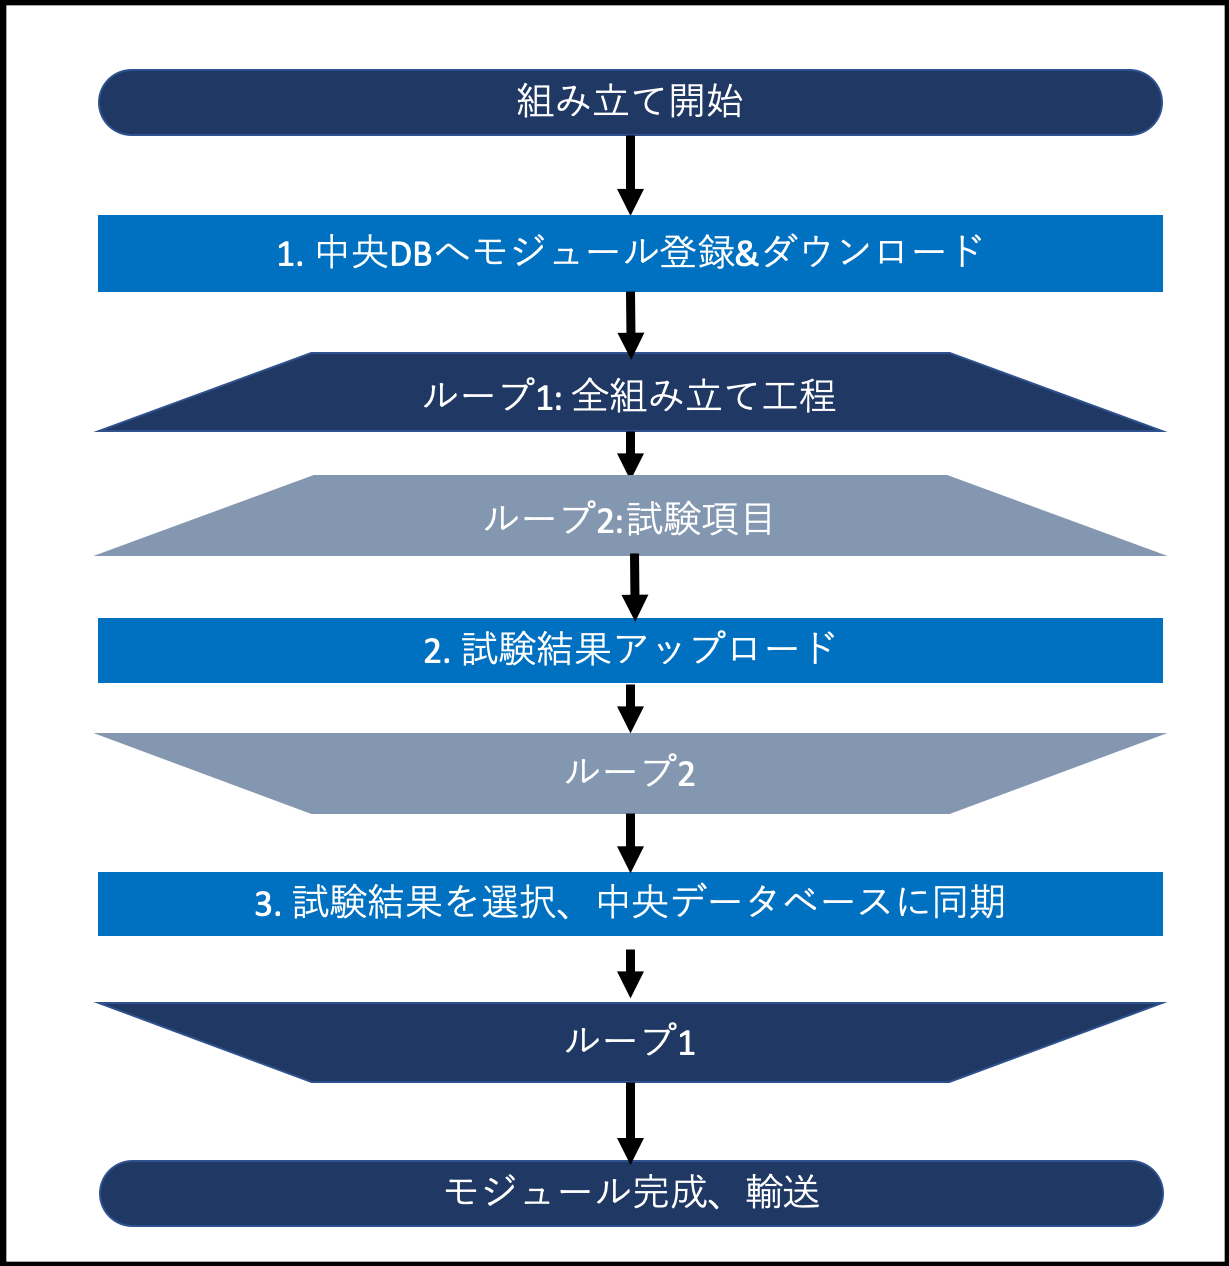
\includegraphics[width=7cm]{./dbsystem_flowchart.png}
  \end{minipage}
  \begin{minipage}{0.4\hsize}
    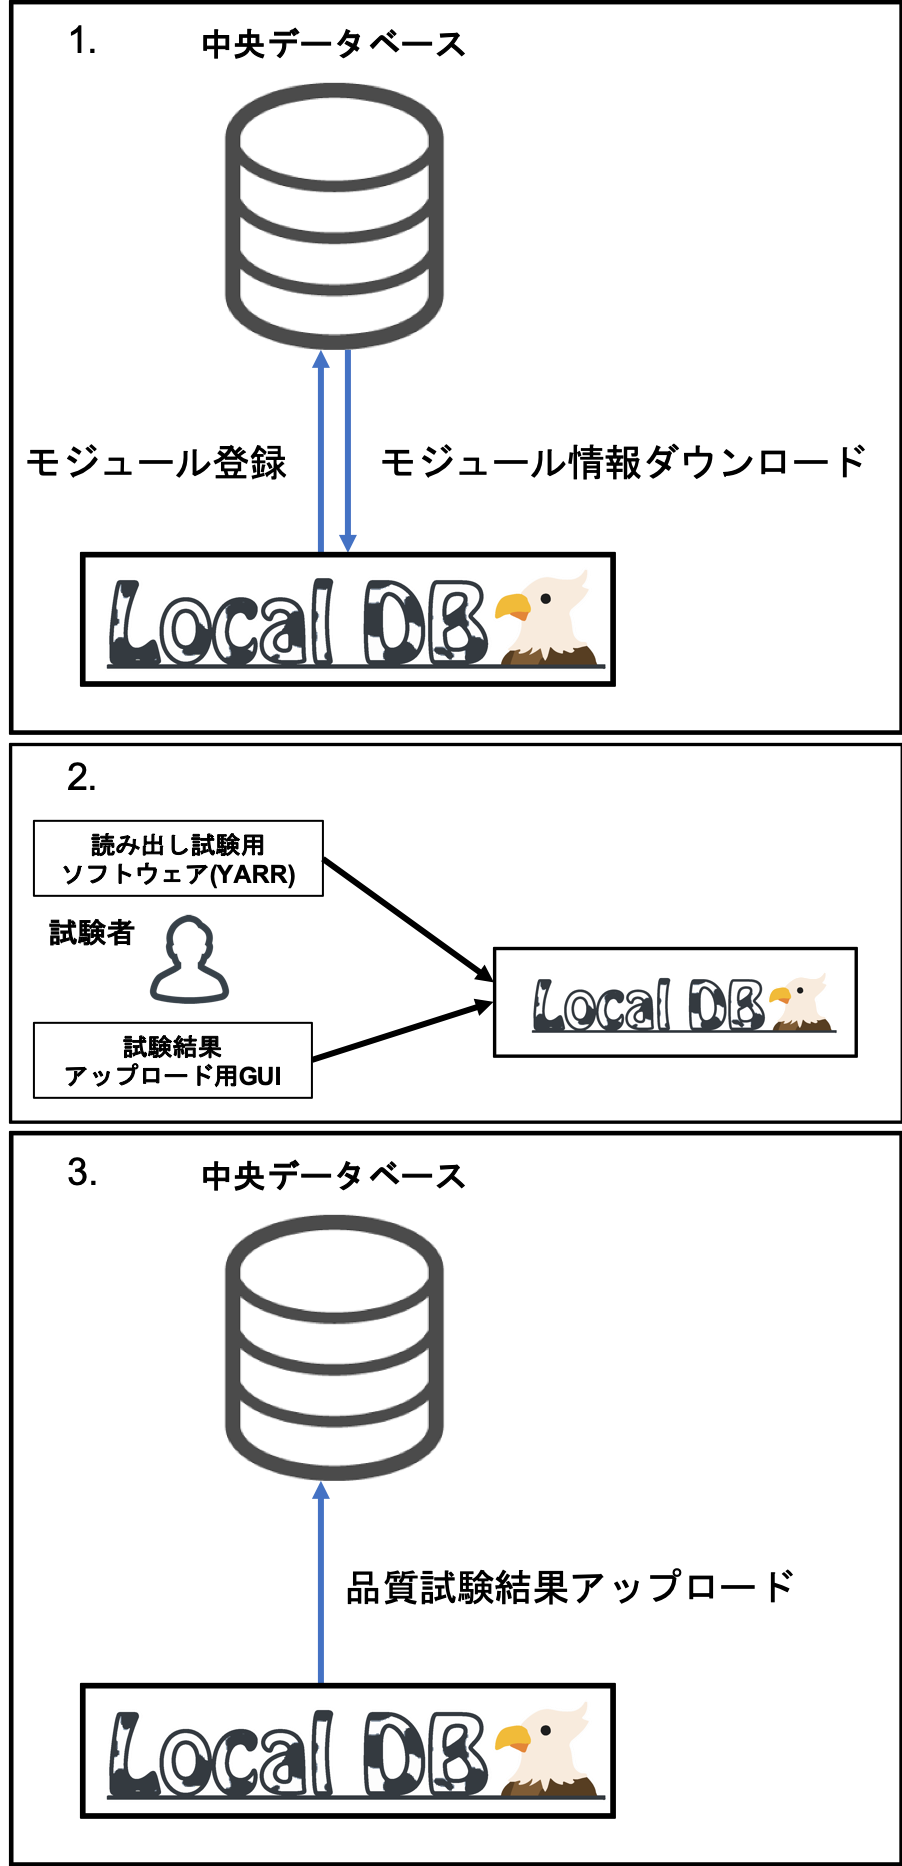
\includegraphics[width=5cm]{./dbsystem_flow_image.png}
  \end{minipage}
\caption[各モジュールにおけるデータベース操作の流れ]{各モジュールにおけるデータベース操作の流れ。モジュール組み立てにおけるデータベース操作の初めに、中央データベースにモジュール登録及びローカルデータベースへモジュール情報のダウンロードを行う(処理1)。その後、ダウンロードしたモジュールに対して組み立て工程に応じた試験結果を生成、ローカルデータベースに保存する(処理2)。各組み立て工程の終わりに試験結果の選択を行い、中央データベースに試験結果を同期する(処理3)。}
\label{dbsystem_flow}
\end{figure}

全組み立て工程が終了すると、モジュールの情報及び品質試験結果が全て中央データベースへ同期されている状態となる。


この品質試験におけるデータベース操作の流れの確立に向けて、2月にCERNに行なったシステムチュートリアルでこの一連の流れを扱った。
ユーザに対する操作方法の周知と機能確認を行うことができた。チュートリアルの概要は付録\ref{cap:appA}に記す。
またシステムのドキュメント\cite{4-7}を作成し、その中に具体的なデータベース操作の流れを記述している。量産時に各機関が適切な流れでデータ管理をできるようにした。


データベース操作の流れの試験として、実際に品質試験のデモンストレーションを行い、各機能が正常に動作するのかの確認を行なった。
詳細を5章で述べる。

